As said in section \ref{subsubsec:Discretization} the simulations are done with the Scalar-weak order 2.0 Ito-Taylor method \cite[algorithm 8.5]{Srkk2019}. The concrete schemes that we derived for the respective types of noises are shown in equations (\ref{eq:OUSim} - \ref{eq:jacobiDiffusion}). All the schemes are implemented in \code{R} and they can be called with specific parameter choices, values for $\tau_c$ and $t_0$ as well as a temporal resolution, $\Delta t$,  and starting point, $x_0$. 

Depending on the $\tau_c$, $t_0$, and $\Delta t$ the method dynamically picks the appropriate number of samples to draw for $\Delta W_k\sim\mathcal{N}\left(0,\Delta t\right)$. The methods allow for positive $\lambda_0$ and negative $A$, but recall that this only correspond to choosing between the positive and negative versions of (\ref{eq:standardStochasticForm}). If no starting point is specified the methods picks the fixed point in the stationary part of the process as the starting point; note that this of course is done with the appropriate branch of (\ref{eq:fixedPoint}) depending on the version of (\ref{eq:standardStochasticForm}), i.e. the sign of $A$. Additionally, an argument is implemented such that we can opt for stopping the process at earlier time (or later) points in time than $\tau_c$. This is useful, when we want to evaluate the models' ability to predict the tipping point based on how far from it we have samples. For details about the timing-benchmarks refer to section \ref{section:benchmark}. Specifications on hardware and software used can be found in table \ref{tab:specs}. 
\subsection{Overview of the estimation methods}
In this section, we test our methods on simulated data. The test aim to illustrate the robustness, computational efficiency and performance in terms of ARE (\ref{eq:ARE}) of the estimation methods. To perform the study for all the models and their respective methods at once, we draw sample paths with the parameters that worked for all models in figure \ref{figure:samplesFromAllDifferentModels}. That is $A = 1.5, m = 0.4, \lambda_0 = -0.2, \sigma = 0.1$; in this part we let $\nu = 1$ and do not estimate this parameter for now. According to the first-order Taylor-expansion, which we use in the stationary part (\ref{eq:TaylorStationary}), the true values here are, $\theta_{\mathrm{stationary}} = (1.095, 0.7651, 0.1)^\top$.  For the dynamic part, we simulate using $t_0 = 30$ and $\tau_c = 30$. We simulate with temporal resolutions $\Delta t = \{1/5, 1/10, 1/25, 1/100, 1/250\}$, corresponding to $N = \{150, 300, 750, 3000, 7500\}$ number of samples in each part of the process. For each value of $N$ we run the simulations and estimation $M = 50$ times and record the median ARE for each parameter. In addition, we calculate the median run-time for each method. In both cases we use the median due to it being more robust against outliers than the mean.

Furthermore, due to the possibility of extreme samples for small $N$; we implement a \code{trycatch}-wrapper around the estimation part such that the program fails gracefully, if estimation should somehow be infeasible for a model on a specific sample. For each run in the simulation all the models are simulated with the same realizations of the brownian motion; if one model fails the all models are re-run using a new seed. The optimizers are initialized at random points where each coordinate can deviate up to $\pm 10\%$ at random from the true values; this is done by sampling three uniform variables according to $U\sim\mathrm{Unif}(0.9, 1.1)$ and multiplying them with the true values. As convergence criterion for the likelihood-based methods we use a relative tolerence of $\code{sqrt(.Machine\$double.eps)/10}\approx 1.49\cdot 10^{-9}$, while the estimation equations that solves their equation numerically use $10^{-8}$ the standard of \code{nleqslv::nleqslv}. 

The likelihood based methods are the MLE and the Strang-based estimators; when there is more than one such method for a specific model, we denote it \textit{Likelihood (Alt.)}. Naturally, estimators based on the score equation or martingale estimation function based equation are estimation equation based estimators together.
\subsubsection{The stationary parts}
In the stationary parts, we run the simulations as described above and depict the median ARE as a function of sample size on a double logarithmic scale
\begin{figure}[h]
    \begin{center}
    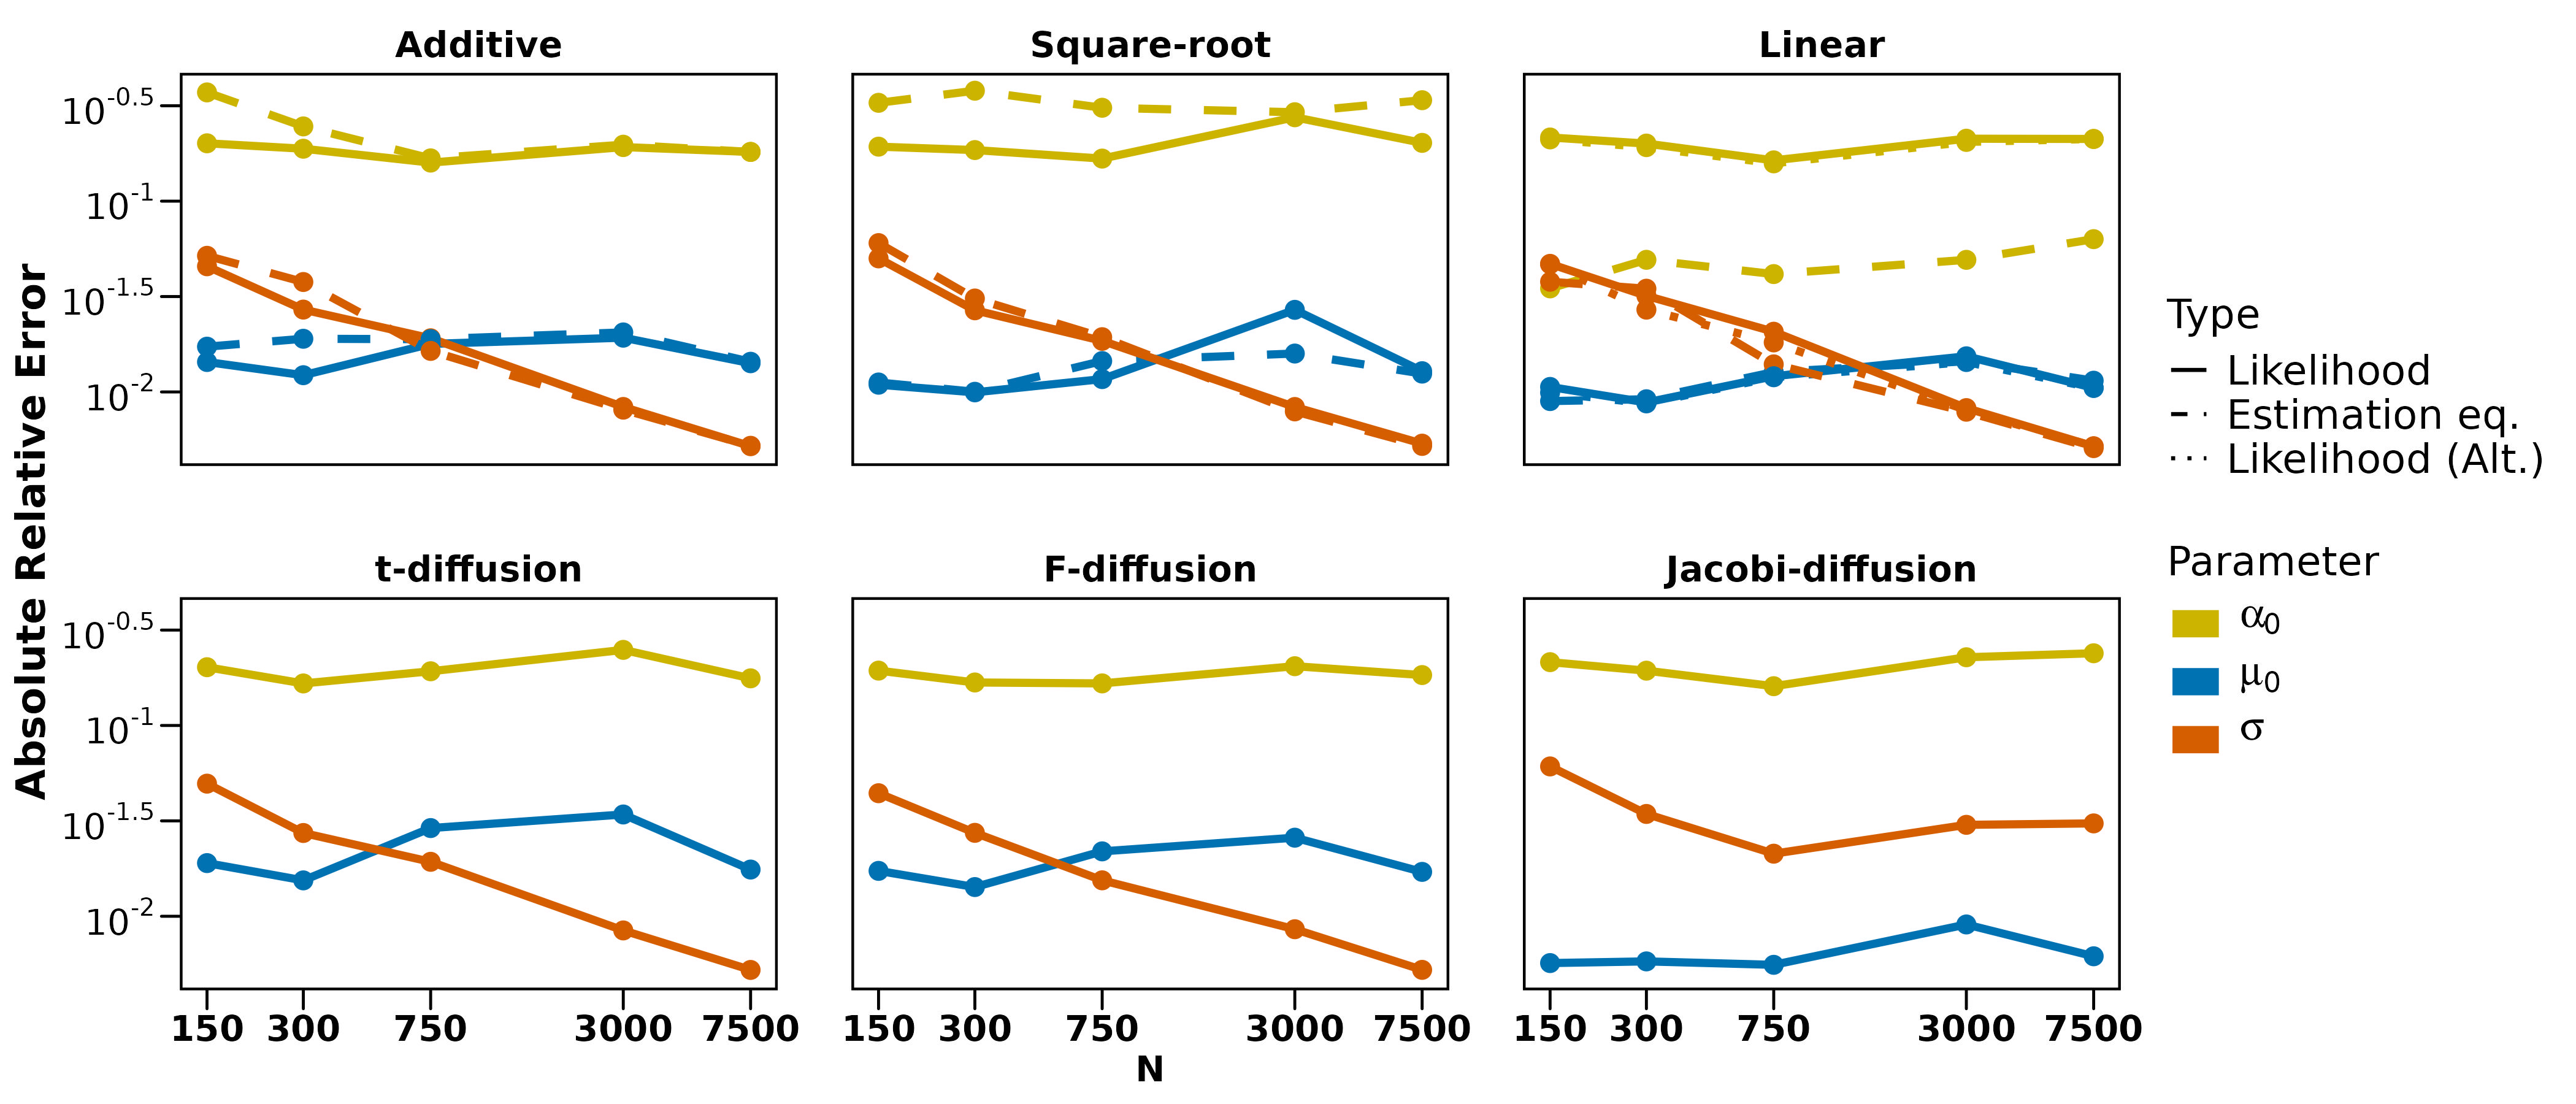
\includegraphics[scale = .1]{figures/parameter_precision_stationary.jpeg}
    \caption{Overview of our estimation methods for the stationary parameters applied to the models}
    \label{figure:overviewOfEstimatorsStationary}
    \end{center}
\end{figure}\\
Note that the specific scale this experiment is done at likely affects the results. The impression of the estimators here likely does not generalized. To see why this might be the case, consider for instance how noisy the additive model is in figure \ref{figure:samplesFromAllDifferentModels} compared to figure \ref{figure:samplesFromFiveDifferentModels}, and then recall that we are in the situation in figure \ref{figure:samplesFromAllDifferentModels}. On the other scale in figure \ref{figure:samplesFromFiveDifferentModels}, the parameters of the additive model might be relatively easier to estimate than the other models.
 
Moving on, we cleary see that the $\alpha_0$-parameter inherently is more difficult to estimate. Additionally, figure \ref{figure:overviewOfEstimatorsStationary} reveals that it is only really the $\sigma$ parameter for which more samples improve the absolute relative error; the other parameters mostly stay at their respective levels in terms of median ARE. The $\mu_0$-parameter is generally not very troublesome to estimate - for any model it consistently has an ARE of around $10^{-2}$ in median, which is around 1.5 orders of magnitude lower than the same metric of the $\alpha_0$-parameter. Still, all the parameters are relatively well estimated in median, indicating that they are quite robust even for starting values that deviates somewhat. Again, this might stem from the fact that the models could behave especially nicely on the unit interval, but the initial test at least do not reveal any significant issues.

For the models with more than one method there is no significant difference in the median ARE of any of the parameters. With regards to $\alpha_0$ in the linear-noise model though the estimation equation faired quite a bit better with an ARE of around an order of magnitude lower than the two Strang based methods. To see how the models compare computationally, we consider the median computation time for the different methods as a function of $N$
\begin{figure}[h]
    \begin{center}
    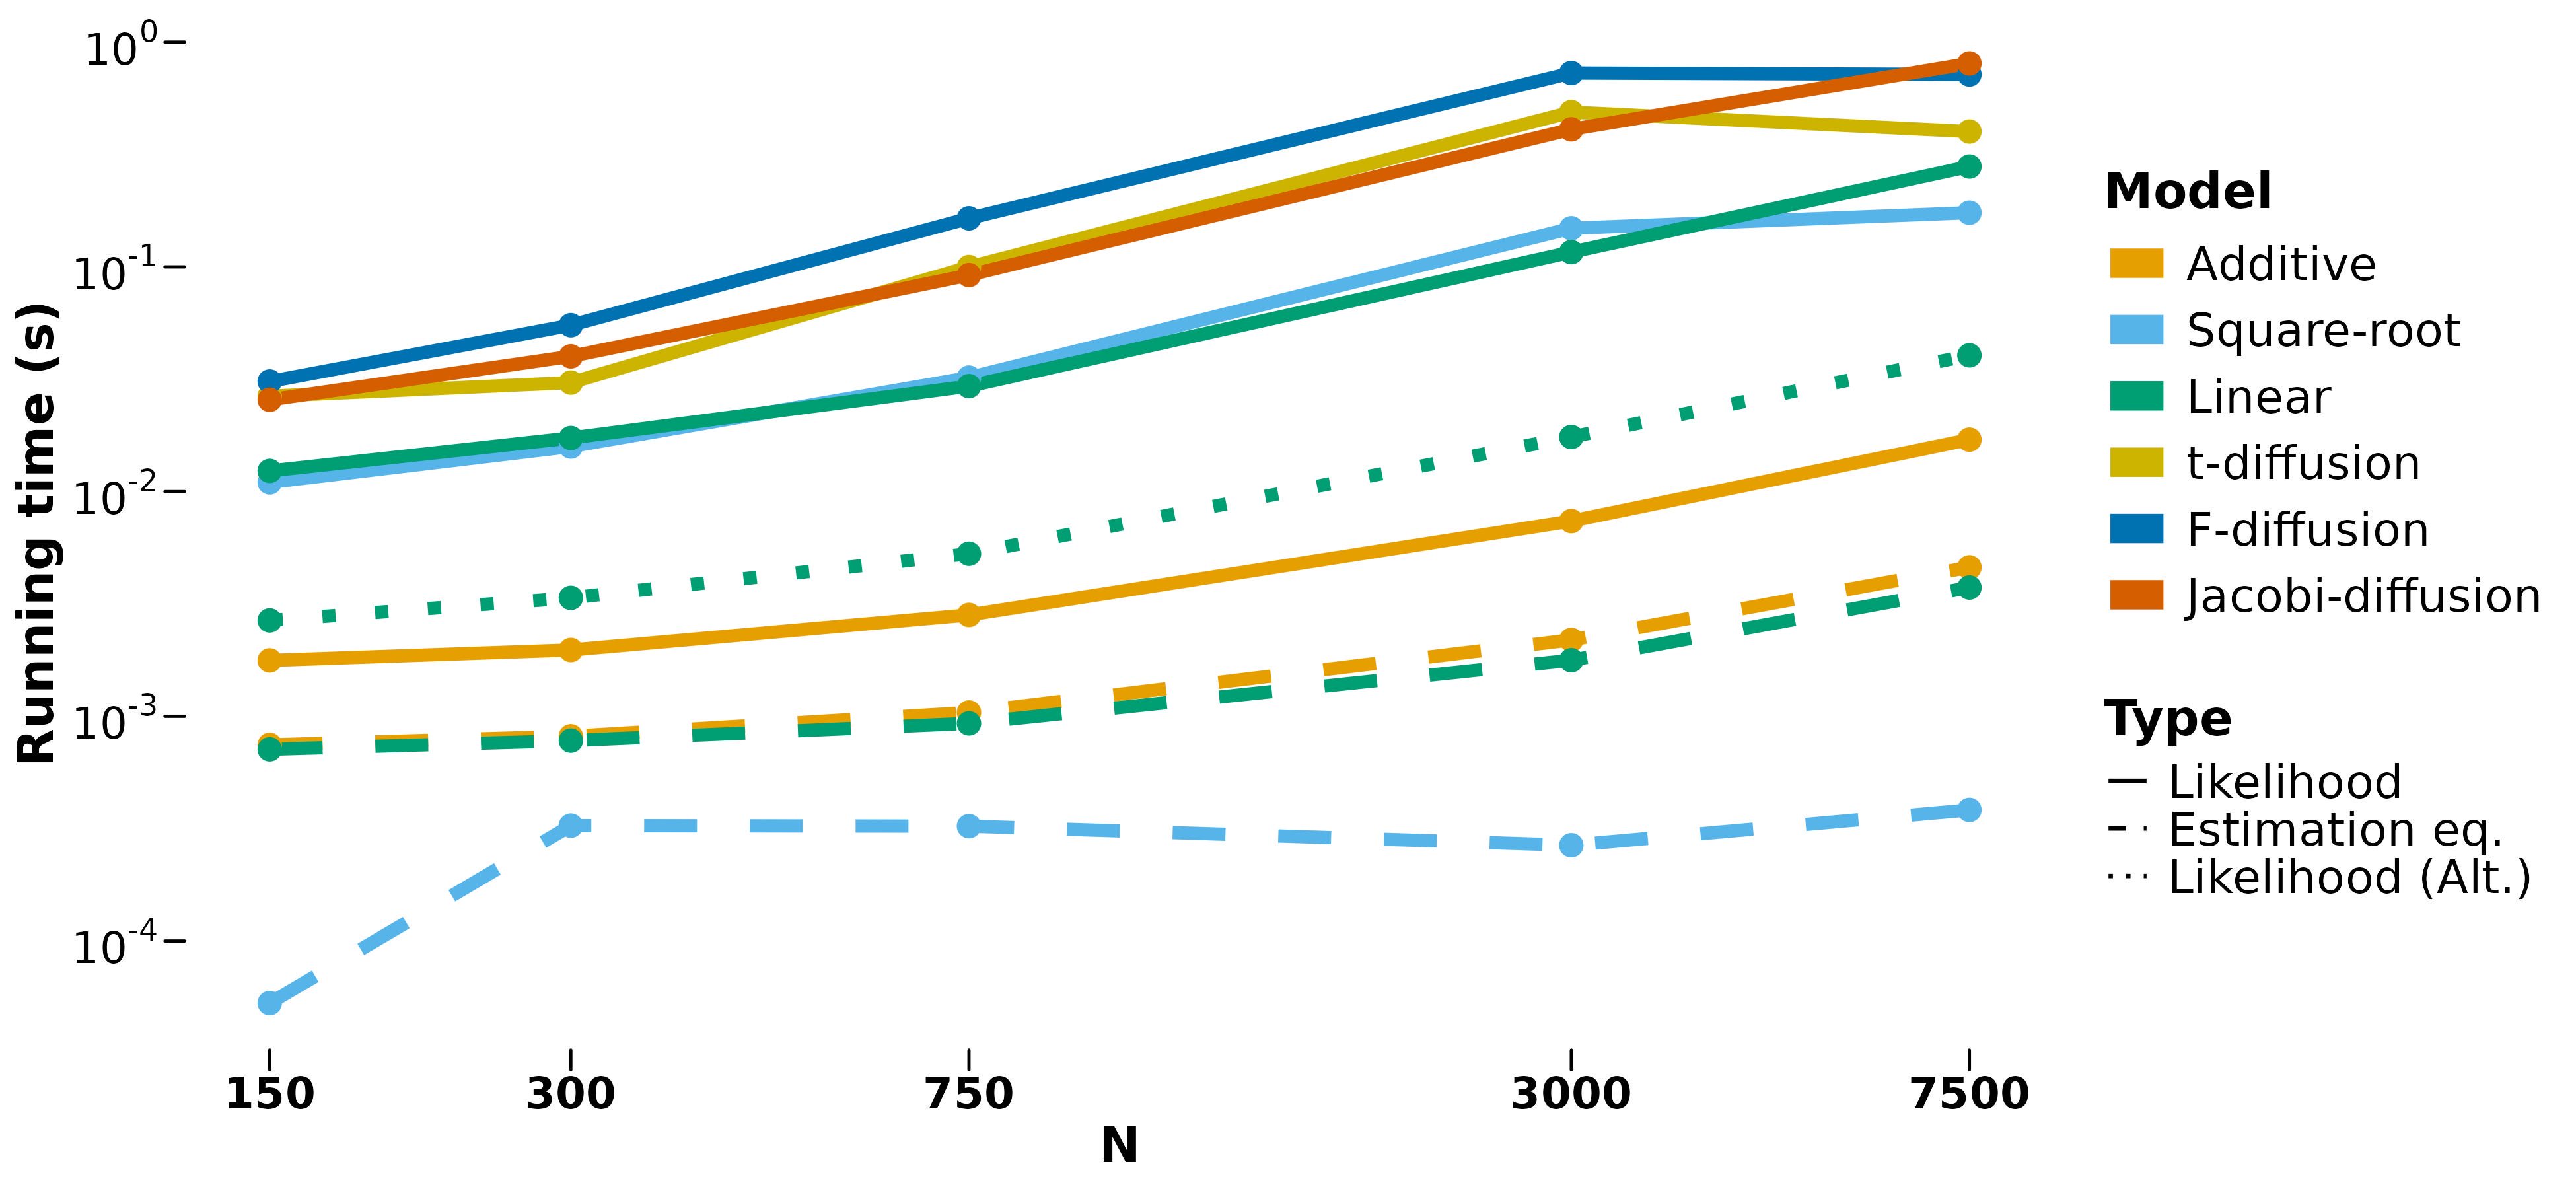
\includegraphics[scale = .1]{figures/estimation_duration_stationary.jpeg}
    \caption{Overview of our the median computation time for each method as a function of the number of samples}
    \label{figure:overviewOfDurationStationary}
    \end{center}
\end{figure}\\
By median computation time we understand the time from the invokation of the optimizer till the convergence criterion is reached. Generally, the estimation equations based estimators are much quicker than the likelihood based, while the explicit estimators based on (\ref{eq:squarerootMartingaleEquation}) for the square-root diffusion are in a league of it owns being between 100 and 1000 times quicker than the likelihood based methods. The latter are generally in the same order of magnitude in terms of performance. Though, the $F$-, $t$- and Jacobi-diffusion based models are slower than the linear and square-root based models. This might be caused by more complicated ordinary differential equations in these models, which the Runge-kutta needs to solve repeatedly; compare the expression in (\ref{eq:squarerootStationarySplit2}) and (\ref{eq:GBM_StrangNonLinearODE_split}) with (\ref{eq:StrangTDiffusion}), (\ref{eq:FscaledSplitting}) and (\ref{eq:jacobiODE}). If we look at the likelihood based methods that solves the ordinary differential equations numerically and contrast their computation time with the ones that are either use MLE or has a closed form solution to the ODE (\ref{meanrevertingGBMSplit1}), it is clear that there is a computational cost to solving the ODE numerically. However, all methods are fast even for the highest amount of samples in the test, $N = 7500$, no single estimator broke the one second barrier in median.
\subsubsection{The dynamic parts}
Turning to investigating the estimation in the dynamic part of each model, recall that we only use variations of the Strang-method for this. If more than one is used, it is denoted \textit{Strang (Alt.)} here. The alternative Strang estimators are the ones that do not use the lamperti-transform, i.e. the two estimators based on (\ref{eq:squareRootSplit2}) and (\ref{eq:GBMSplit2}) used in the square-root- and Linear models, respectively. We simulate from the models and fit in the manner described above. The ARE of the parameters in the dynamic part is depicted as a function of $N$ using a double logarithmic scale 
\begin{figure}[h!]
    \begin{center}
    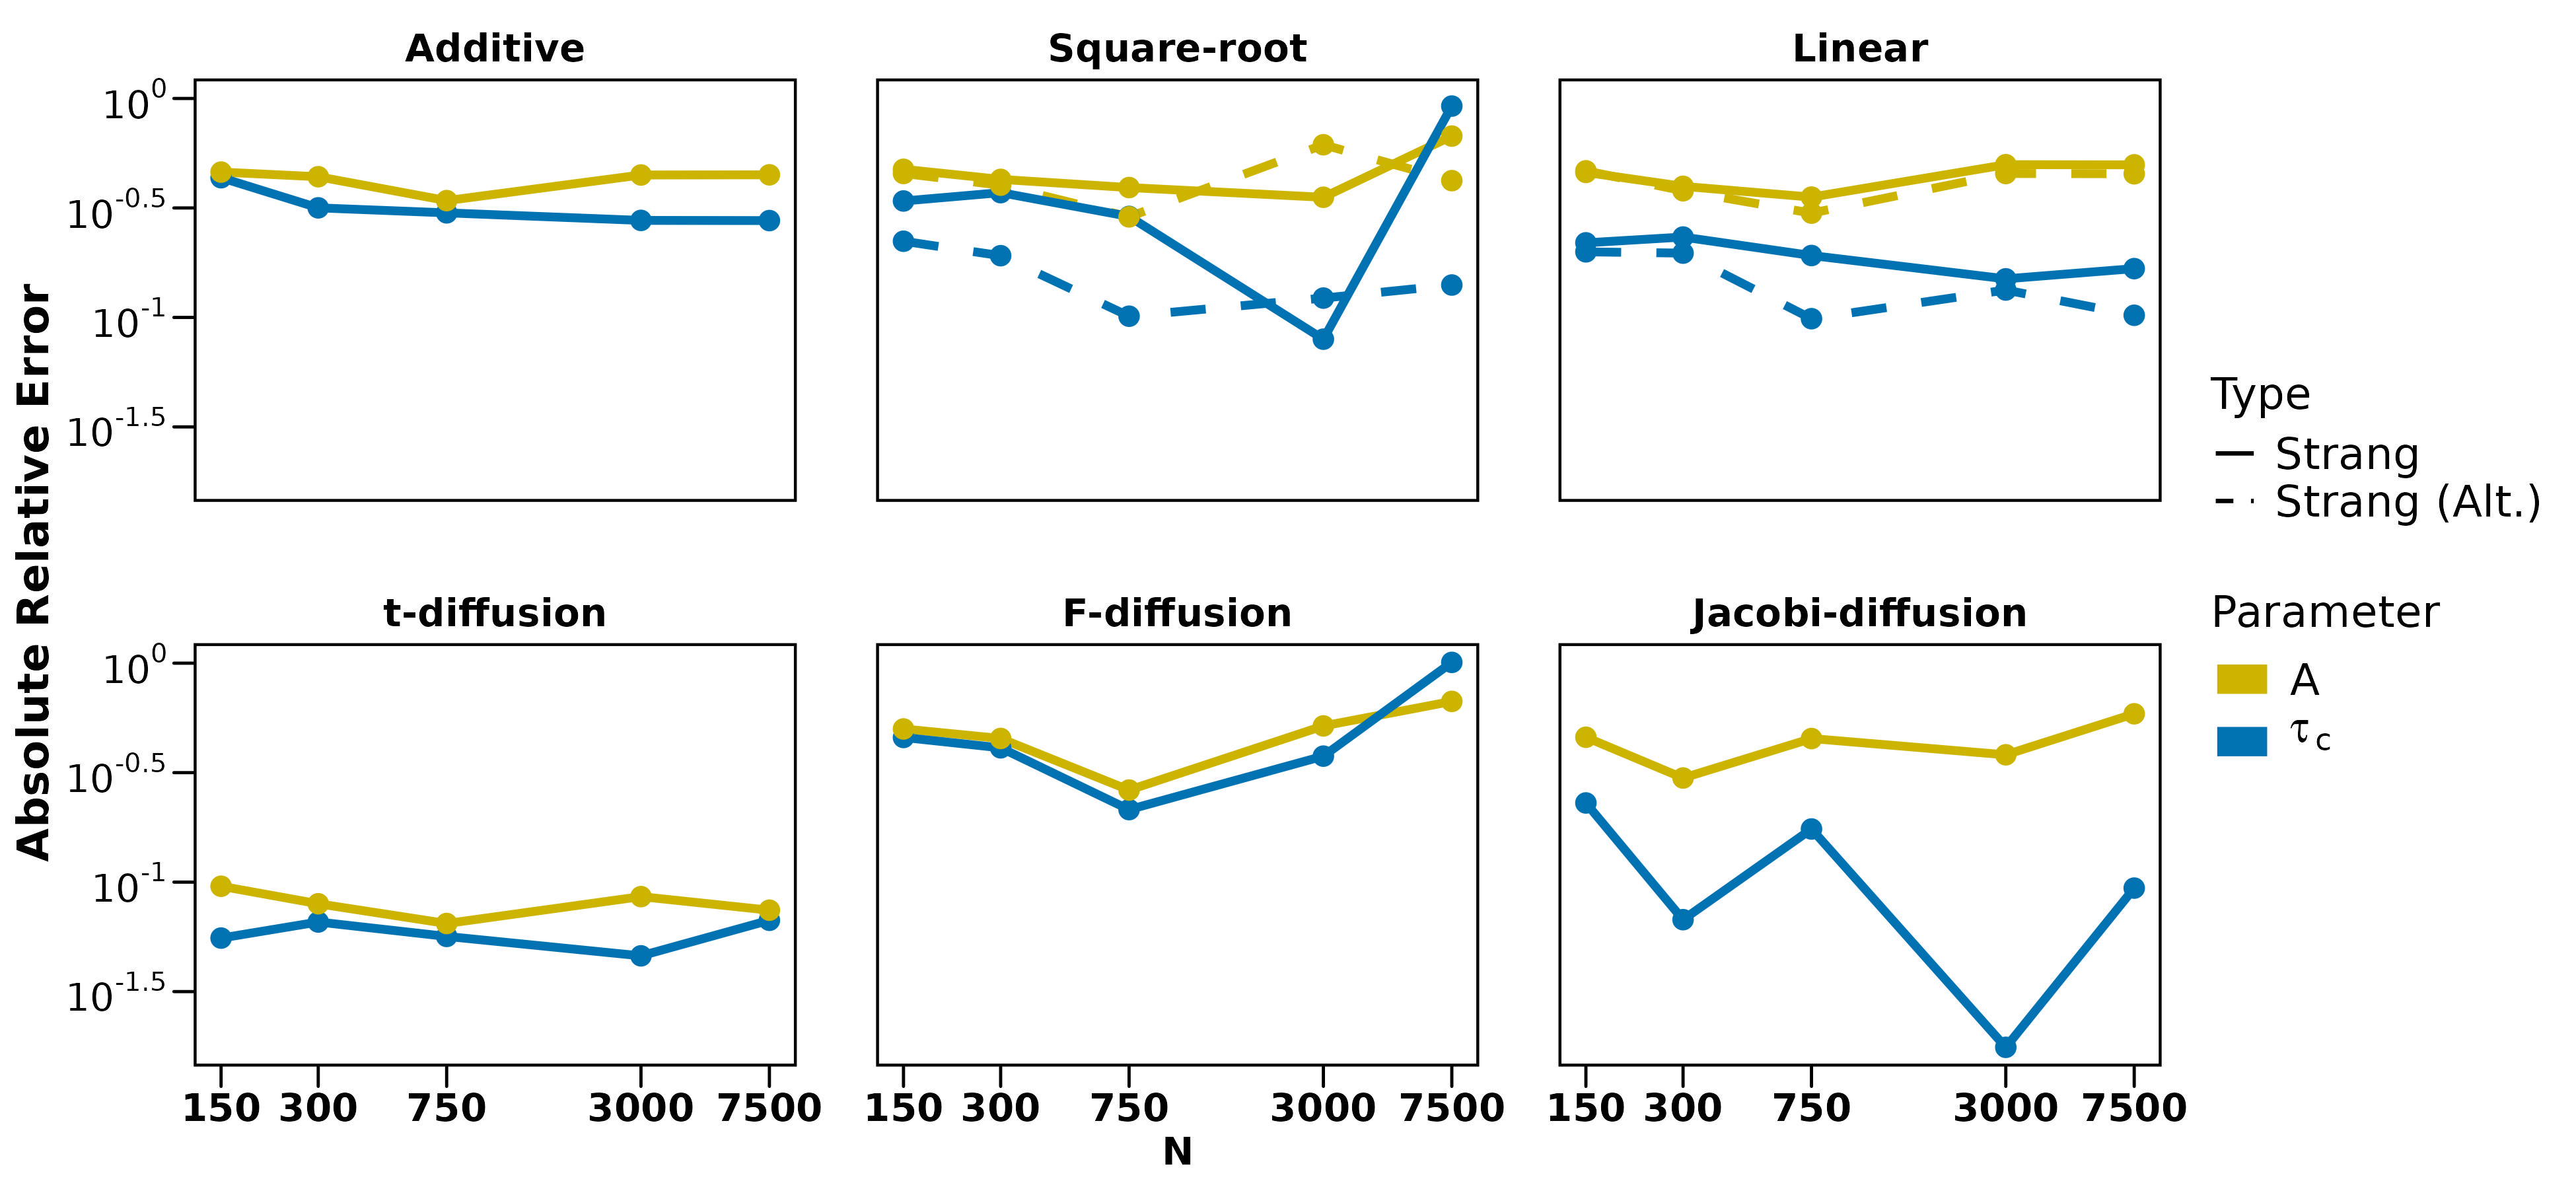
\includegraphics[scale = .1]{figures/parameter_precision_dynamic.jpeg}
    \caption{ARE of the parameters of the models in the dynamic part}
    \label{figure:parameter_precision_dynamic}        
\end{center}
\end{figure}\\
Due to the strong non-linear effects is generally harder to estimate in the dynamic part. In terms of the $A$-parameter all models and type of methods faired relatively equally in terms of ARE. That is with the exception of the $t$-diffusion model, whose ARE are around half an order of magnitude smaller than that of the mother models. For some reason, the normal Strang estimator in the Square-root model as well as the $F$-diffusion based model show a relatively high median ARE for the largest number of samples we investigated.  Considering the other sample sizes this is more surprising for the Square-root noise model, as it is generally easier to estimate in. The $F$-diffusion seems, on this scale at least, to be the hardest of the models to do estimation on; whereas, as we mentioned, the $t$-diffusion based model seems the easiest. 

In terms of overall run time, we achieved similar results in terms of which kinds of models had faster convergence as we saw in figure \ref{figure:overviewOfDurationStationary}. For this reason, the results are only shown in appendix \ref{section:benchmark} in figure \ref{figure:estimation_duration_dynamic}. One surprise from this benchmark though, is the fact that $t$-diffusion based model, which solves its ODE numerically, has the fastest convergence of all the models. This probably stem from the model requiring less iterations overall before convergence is reached, as solving the ODE with Runge-kutta is much more computationally expensive than just computing the solution.
\subsection{Fitting the \texorpdfstring{$\nu$}{nu}-parameter}
We now consider how introducing the $\nu$-parameter into the model affects the performance of the optimizers. For simplicity, we focus on the additive- and t-diffusion based models in this experiment. We ensure that the Brownian motions in a specific run in the simulation are the same. We simulate from both models using $t_0 = 54$ and $\tau_c = 132$ and temporal resolutions $\Delta t = \{1/3, 1/5, 1/25, 1/50, 1/100\}$, which correspond to $N_\mathrm{dynamic} = \{396, 660, 3300, 6600, 13200\}$ samples in the dynamic part. The dynamic part is the important one here, because this is where $\nu$ is estimated. Of course, the quality of the estimates in the dynamic part hinges somewhat on the estimates from the stationary part.

The other parameters are $\theta = (0.87, -1.51, -3,  0.387)^\top$. Due to its non-central role estimation in the stationary part is merely initialized in the true parameters there, and the estimates passed onto the optimizer in the dynamic part. In the dynamic part, optimization is initialized in a similar manner to earlier experiments. We add $\pm 10\%$ multiplicative noise to the true values of $A$ and $\tau$ by sampling two uniform variables according to $U\sim \mathrm{Unif}(0.9,1.1)$. The last parameter $\nu$ is always started in $1$, regardless of the true value. This is done to simulate the user assuming the more parsimonious with $\nu = 1$ and then letting the data show that $\nu$ is something else. 

For each value of $\Delta t$ we investigate how the models and optimizers perform on $\nu_{\mathrm{sim}} = \{0.75, 0.9, 1, 1.11, 1.33\}$. For each combination we run $M = 50$ simulations. As earlier, we consider the median of the ARE for each combination of $\Delta t$ and $\nu$. The experiments are once more implemented such that failure to converge or run the optimization results in a graceful exit. Now, instead of merely retrying after a failed optimization attempt, we count how many time each model fails for every combination of $\Delta t$ and $\nu$. This is to highlight, if there is a specific model or parameter value of $\nu$ that is troublesome to estimate on. The relative tolerance convergence criterion in \code{optim} was set to \code{sqrt(.Machine\$double.eps) / 1000} to avoid getting stuck in local minima. 

We start by considering the ARE 
\begin{figure}[h!]
    \begin{center}
        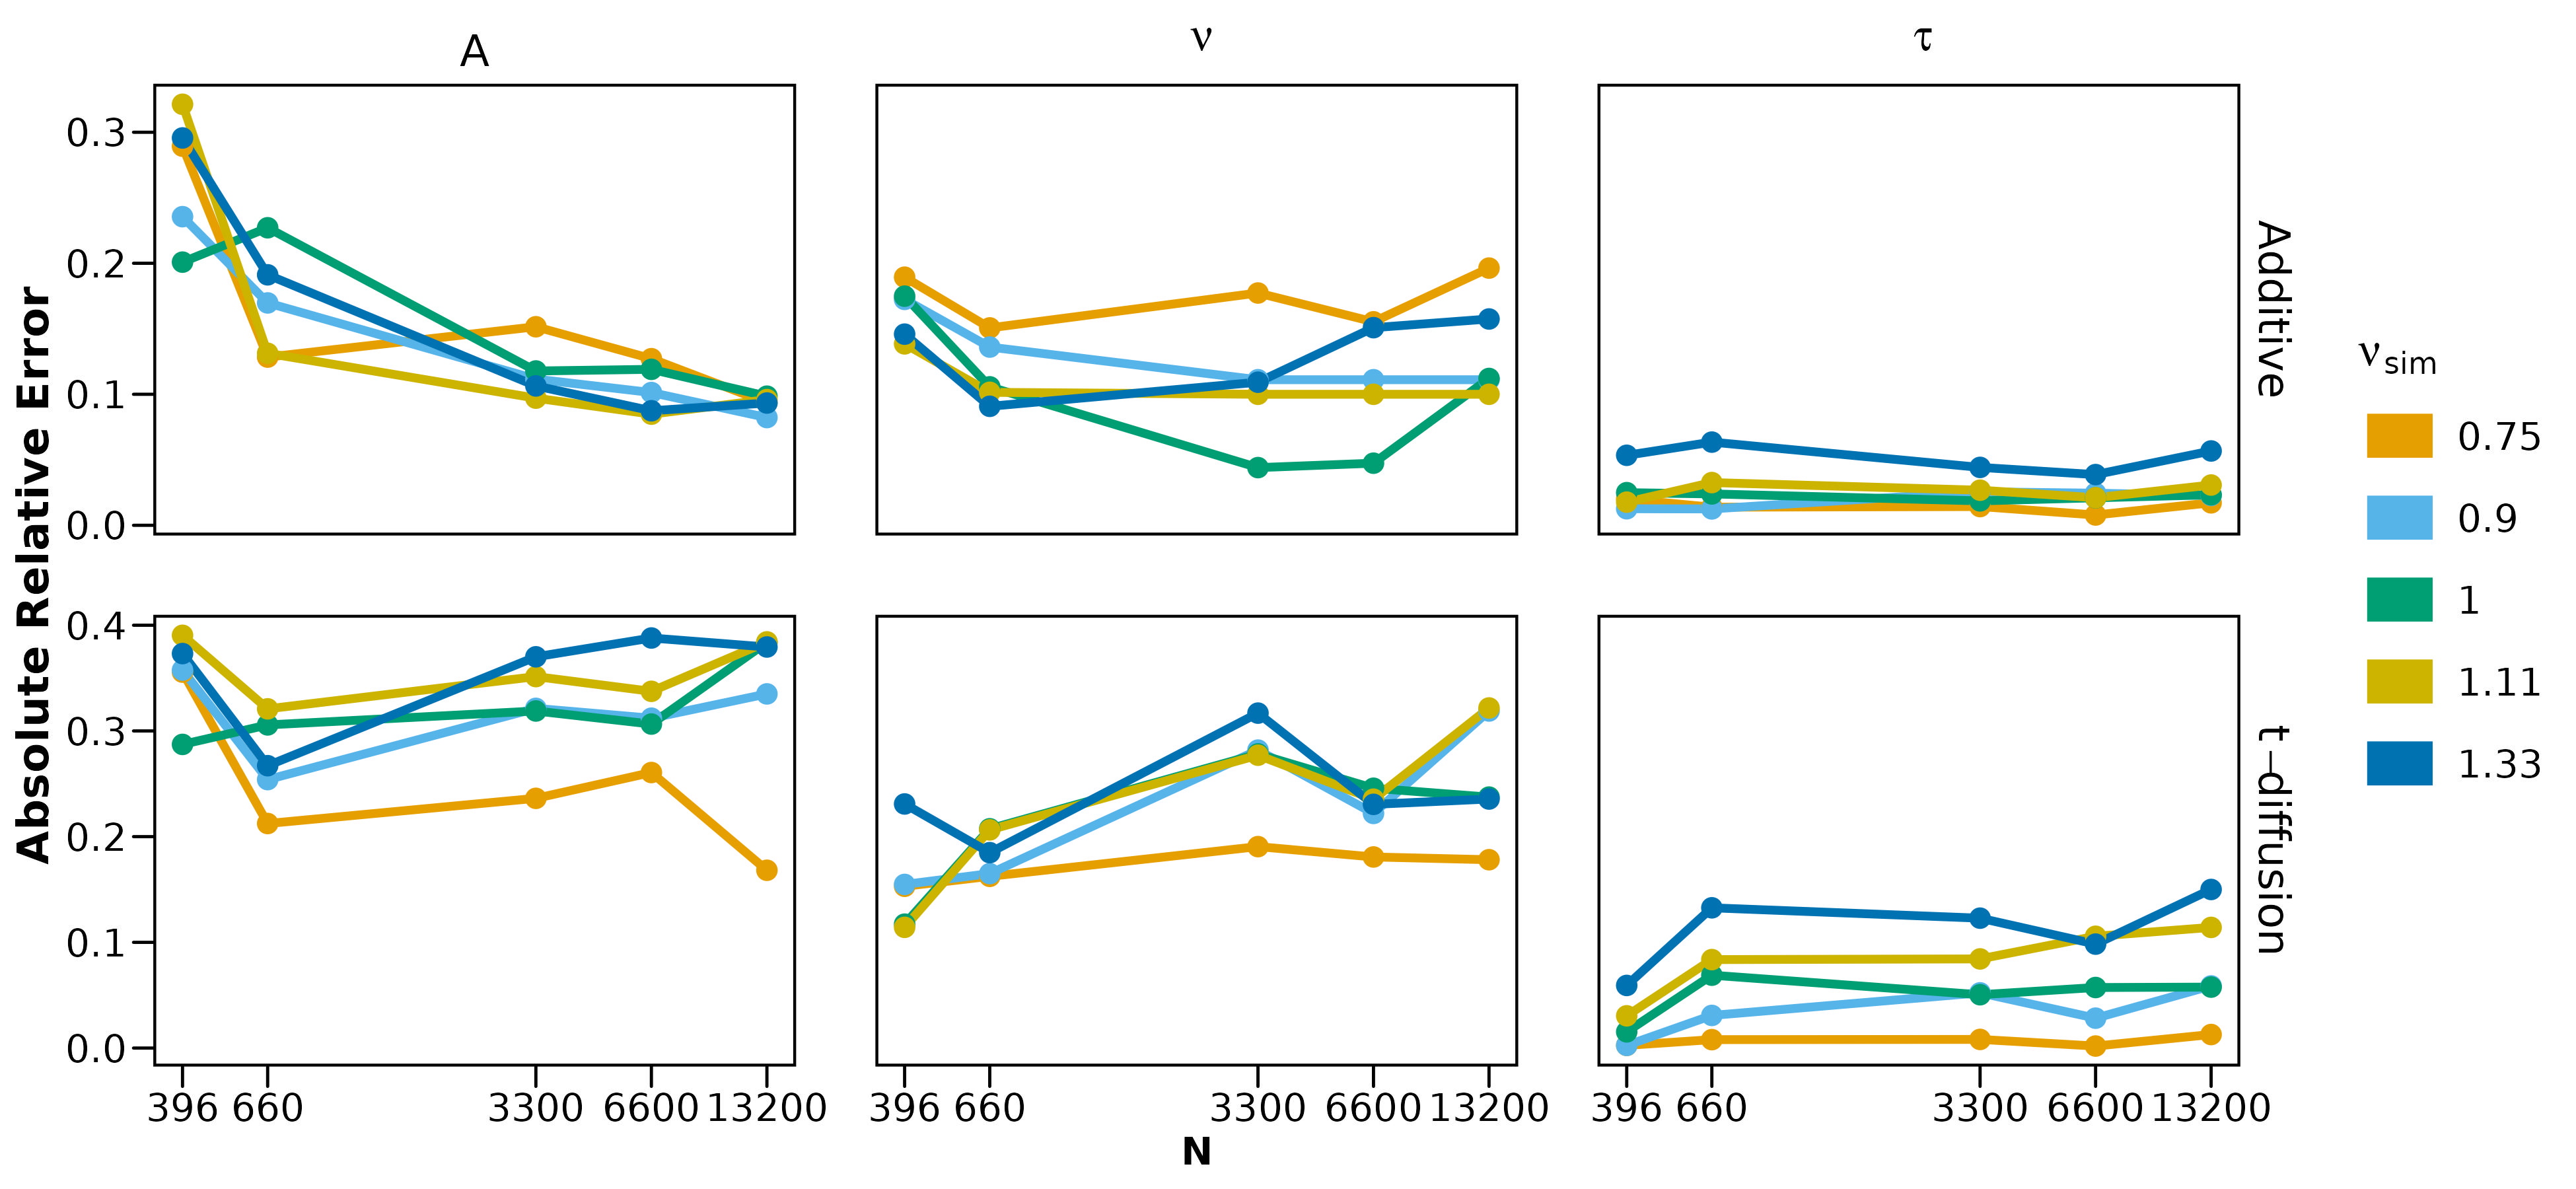
\includegraphics[scale = .1]{figures/combined_nus_plot.jpeg}
        \caption{The absolute relative error of the different parameters as a function of $N$ for diffferent true values of $\nu$.}
        \label{figure:ARE_nu_plots}
    \end{center}
\end{figure}\\
Note that the $x$-axis is logarithmic in figure \ref{figure:ARE_nu_plots}. From the graph we see that increasing the number of samples only really makes the median ARE better for the model with additive noise and only considerably for the $A$-parameter. Though, the median ARE for the other parameters are generally low. Increasing the true value of the $\nu$-parameter, does result in an overall larger ARE. If we look at figure \ref{figure:nu_plot}, this is not too surprising. As we also commented on the graph, increasing $\nu$ results in the two fixed points being closer to one another longer before the bifurcation point. This creates a situation, where the process tips due to noise more frequently - thus making it difficult to estimate when bifurcation tipping would occur. All in all, though, the values depicted here does not seem to alarming considering the added flexibility having a $\nu$-parameter provides. However, they do not constitue the full picture themselves; we also counted how many times each method failed during optimization - yielding the following results
\begin{figure}[h!]
    \begin{center}
        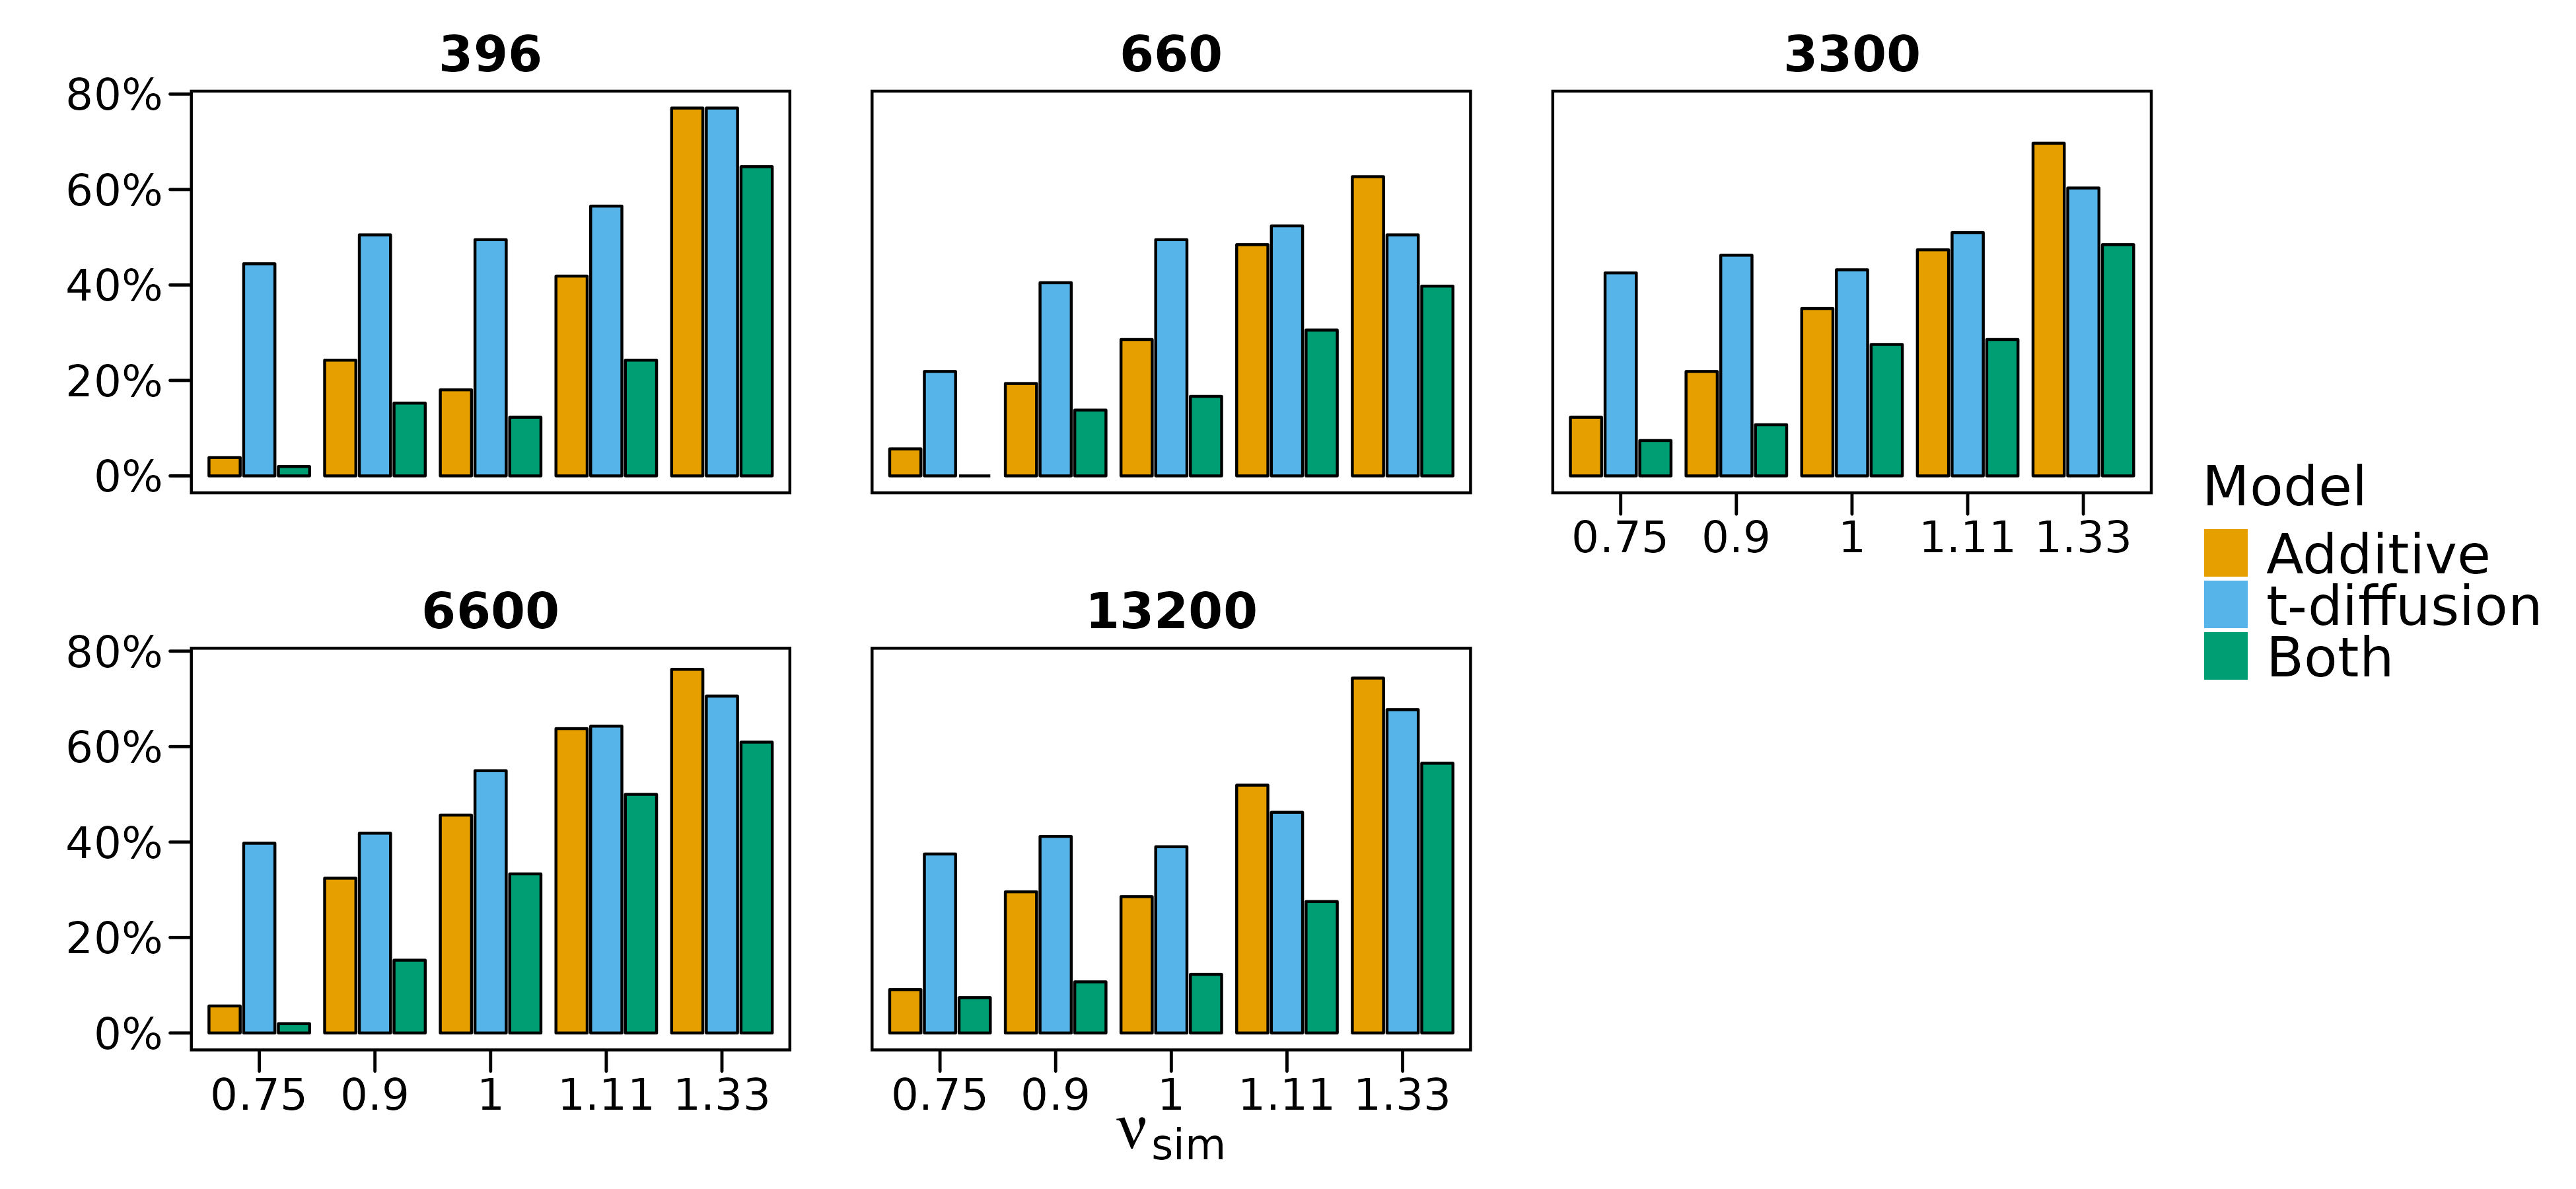
\includegraphics[scale = .1]{figures/error_count_plot.jpeg}
        \caption{The proportion of times where the respective models or both failed doing optimization as a function of $N$ and for different true values of $\nu$.}
        \label{figure:error_count_nu_experiment}
    \end{center}
\end{figure}\\
Keep in mind that the $x$-axis is now $\nu_{\mathrm{sim}}$, whereas the individual elements in the grid correspond to graphs for different values of $N$. Evidently, estimating with $\nu$ in the model estimation fails quite frequently. This is even when we a provided with estimates from the stationary part, where optimization was initialized in the true values. In comparison, we have virtually never during testing experienced the methods fail to optimize, when we only opt for estimation of $A$ and $\tau_c$ in the dynamic part. Now, the model with additive noise faires better overall and it seems that as long as the true value $\nu\leq 1$ the is a reasonable chance of success with it. Though, this provides little consolation, as we do not know this in actual applications. Furthermore, we would, of course, like to be able to estimate in models with $\nu > 1$ too.

At the same time, the models do not seem to do better for larger sample sizes unfortunately. In addition, the $t$-diffusion based model has for all samples sizes at least a $20\%$ chance of failing, which is unacceptable. From the green bar it is also rather clear that whenever the additive models does fail, it is often the case that the $t$-diffusion based model fails as well.  
%\subsection{Early warning analysis}
\subsection{The numerical Strang}
We introduced the idea of the numerical Strang splitting in section \ref{subsection:NumericalStrangSplitting}. In sum, the aim was to numerically do as many of the computations to make a Strang splitting scheme that follows the heuristic in \cite{SplittingSchemes} as possible. The implementation we ended up with only needed to be provided the lamperti transform and the drift of the Lamperti-transformed SDE, and then it would take care finding fixed points, constructing the linear SDE etc. In this section, we constrast the numerical Strang applied to two models with their respective analytical counterparts. The ones we consider are the model with linear noise and the F-diffusion based model. 
These models have their ODE solved numerically, meaning that in the terms "analytical" and "numerical" should be understood relatively. For clarity we will instead in the following refer to the "analytical" method as \textit{closed-form} alluding to the fact that it is the one where we use the closed form solution of the fixed point For their lamperti-transform confer table \ref{table:ergodicDiffusions}, while the lamperti drifts can be found at (\ref{eq:GBM_lamperti}) and \ref{eq:F_diffusion_lamperti_SDE}. Because of the time dependence of the fixed points through $\lambda_t$ in the dynamic parts, we did not consider these, as it would be much more difficult to implement a method that finds a fixed point for each time-point in a process. However, we later discuss how one could potentially overcome this obstacle.

We simulate using $A = 1.5$, $m=0.4$, $\lambda_0 = -0.2$ and $\sigma =0.15$ as well as $t_0 = 30$ with temporal resolution $\Delta t = \{1/5, 1/50, 1/150, 1/500, 1/1000\}$, which in other words means: $N =  \{150, 1500, 4500, 15000, 30000\}$.  The parameters correspond to $\alpha_0 = 1.095$, $\mu_0 = 0.7651$ and $\sigma = 0.15$ for the true parameters of the stationary part; these are the parameters we want to estimate. For each value of $N$, we run $M = 50$ simulations, do estimation and time the estimation with \code{microbenchmark}.

Optimization is initialized at noisy starting values as previously. This time the uniform variables are sampled such that each coordinate has a deviation from the true value of up to $\pm 25\%$ at random; though as before this noise is the same for all methods in a specific run of the simulation. As convergence criterion we use the standard in \code{optim}: \code{sqrt(.Machine\$double.eps)}. We let the methods fail gracefully, but again keep track of how many time each method fails. Apart from this metric, we consider the distribution of the ARE to get a detailed view of how the methods perform - also in the extreme case. In this section, the results are shown for the model with linear noise as our findings are the most clear in this model. Still, the same results as we are about to show, can be found for the $F$-diffusion based model in figure \ref{figure:ARE_dist_numeric_F_diffusion} in appendix \ref{section:benchmark}. For the linear model, though
\begin{figure}[h!]
\begin{center}
    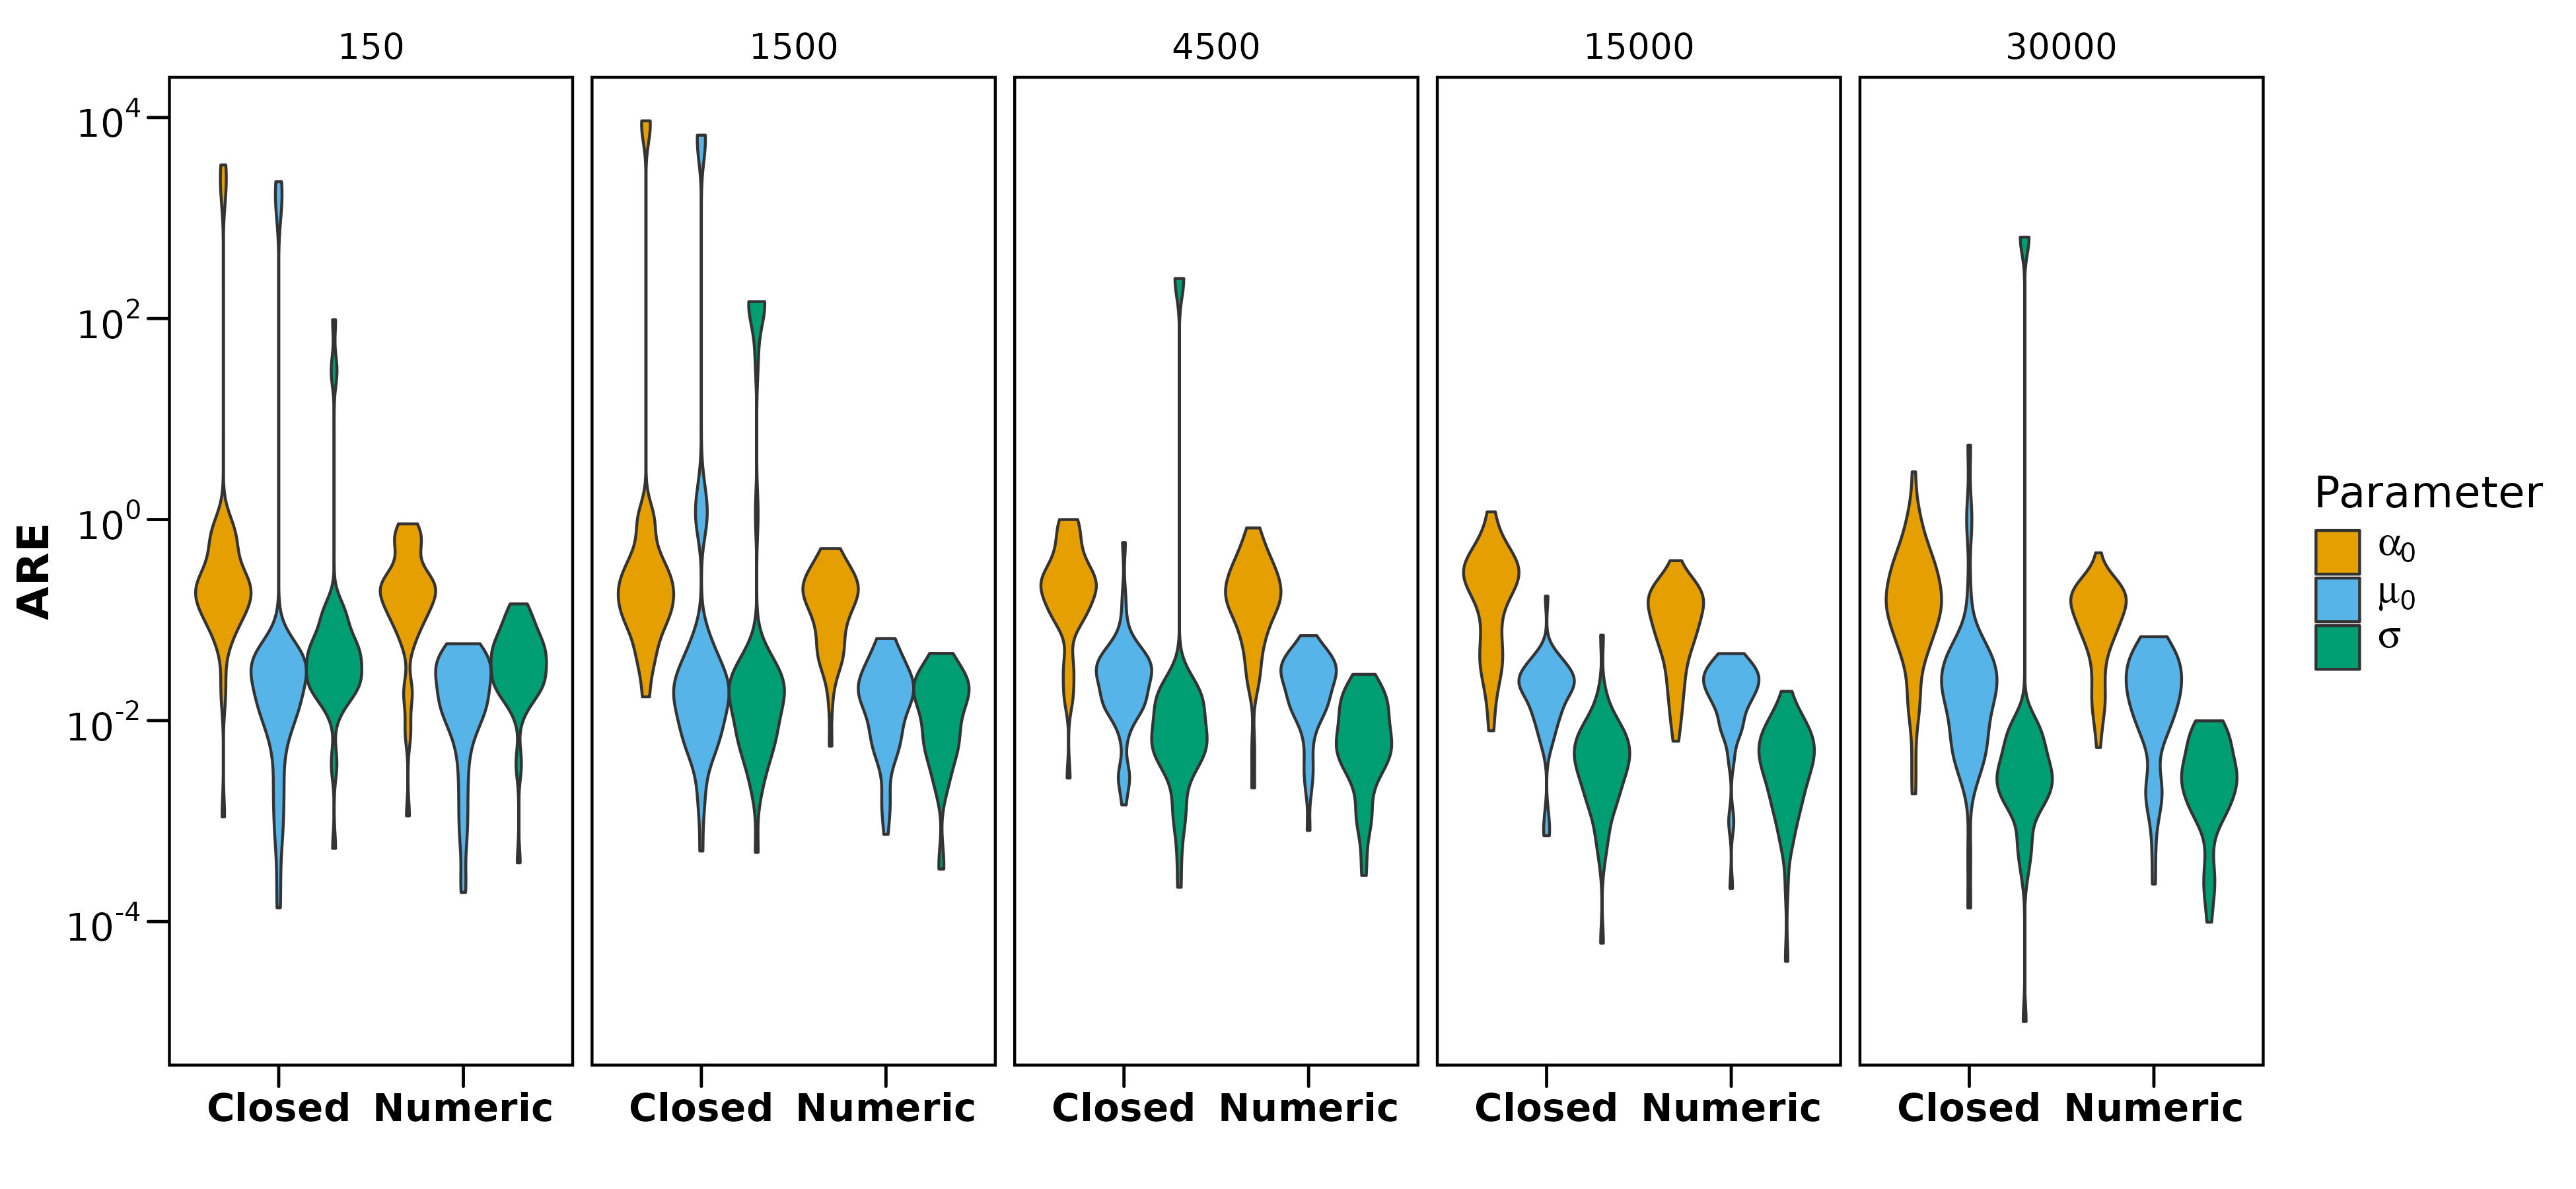
\includegraphics[scale = .1]{figures/ARE_dist_result_plot_Linear.jpeg}
    \caption{Distribution of the ARE of the parameters in the linear noise based model shown for the numerical- and closed form type estimation methds.}
    \label{figure:ARE_dist_linear_noise}
\end{center}
\end{figure}\\
Initially, it is worth mentioning that across all runs in both models, it was only the closed form solution of the linear-model that ever failed to optimize. It did this around $20\%$ of the time for $N = 150$; $2\%$ for $N = 4500$ and $4\%$ for $N = 30000$, but never at other $N$. This fact aligns well with the results depicted in figure \ref{figure:ARE_dist_linear_noise} as it suggests a lack of overall robustness of the method. In the graph we see that there are a few quite extreme ARE-observations for parameters estimated by the closed form method. Conversely, a general better performance of the numerical estimator is evident by the fact that the distribution of the ARE for a specific parameter and fixed number of samples is shifted towards zero for this estimator. 

Now, these results clearly speak for the numerical method. However, it is not difficult to come up with a potentially significant drawback of this method: Finding the fixed point, evaluating this point in the derivative of the drift via a finite difference based method to then construct the ODE in the Strang splitting in a way where we cannot exploit any potential simplifications that might arise in the analytical expressions is bound to give us a method that is slower than the closed-form solution. Benchmarking the two methods for both models over the same runs that gave the results shown in figure \ref{figure:ARE_dist_linear_noise} and - \ref{figure:ARE_dist_numeric_F_diffusion} yields the following run-times
\begin{figure}[h!]
    \begin{center}
    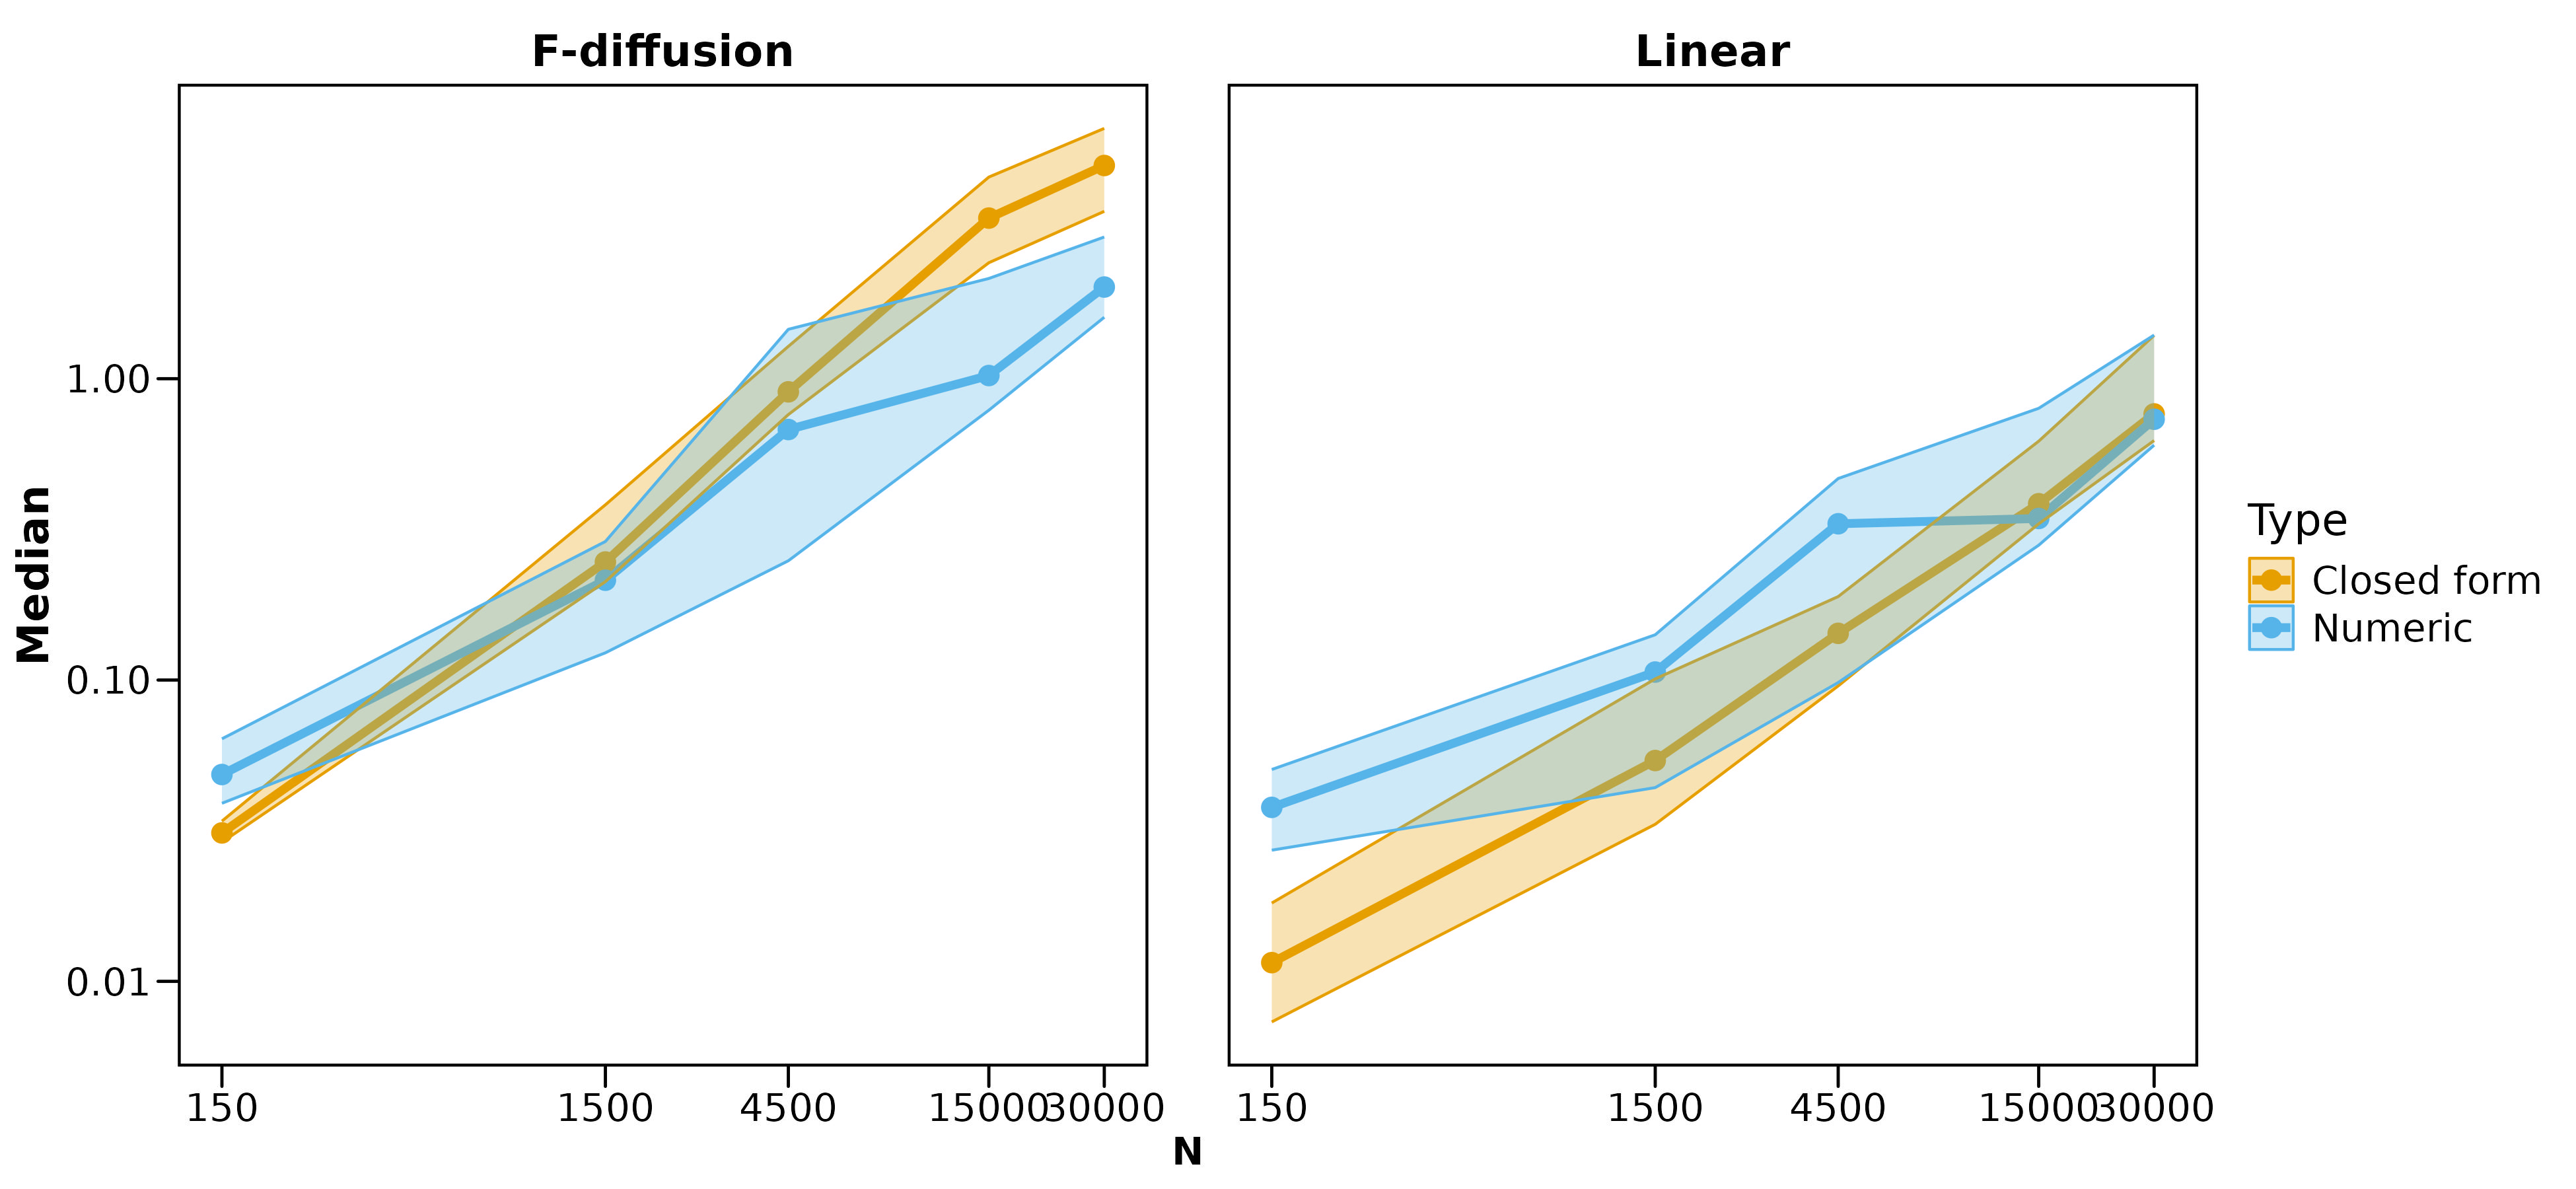
\includegraphics[scale = .09]{figures/Running_result_numeric.jpeg}
    \caption{Running-times for the Linear-noise- and $F$-diffusion based models stratified after type of Strang method.} 
    \label{figure:running_result_numeric}       
    \end{center}
\end{figure}\\
The borders of the shaded region constitute the $10\%$ and $90\%$ quantiles of the run-times, while the solid line is the median run-time. Also, note that figure \ref{figure:running_result_numeric} is double logarithmic. Initially, we see what we might expect, the Numerical method has a relatively slow convergence in comparison to the closed form solution. However for larger samples this picture shifts completely for the $F$-diffusion, whereas the method is on par with the closed-form method in the Linear-noise model. This is a bit surprising as each call of the numerically based objective function needs to do many more operations. Not only that but we also have to factor in the overhead of calling \code{nleqslv::nleqslv} and \code{numDeriv::grad} repeatedly. The added overhead might explain why the numerical methods are slower for smaller sample sizes as the overhead cost of a function call make up more of the total run-time in these instances. The effect of this added cost is negligible when the program spends more time doing actual computations. Still, the computations themselves should be slower even when we have more samples. 

To see where the numerical method might gain its edge in terms of speed of convergence, though, we counted the number of times the methods had to evaluate the objective in order to find the minima. The \code{counts} output from \code{stats::optim} returns the number of evaluations of the gradient and function that was required for a specific run to convergence. Facetting over $N$, we depict this distribution for the Linear noise model grouped after what \textit{Type} of evaluation the objective used. We get the following distribution
\begin{figure}[h!]
    \begin{center}
    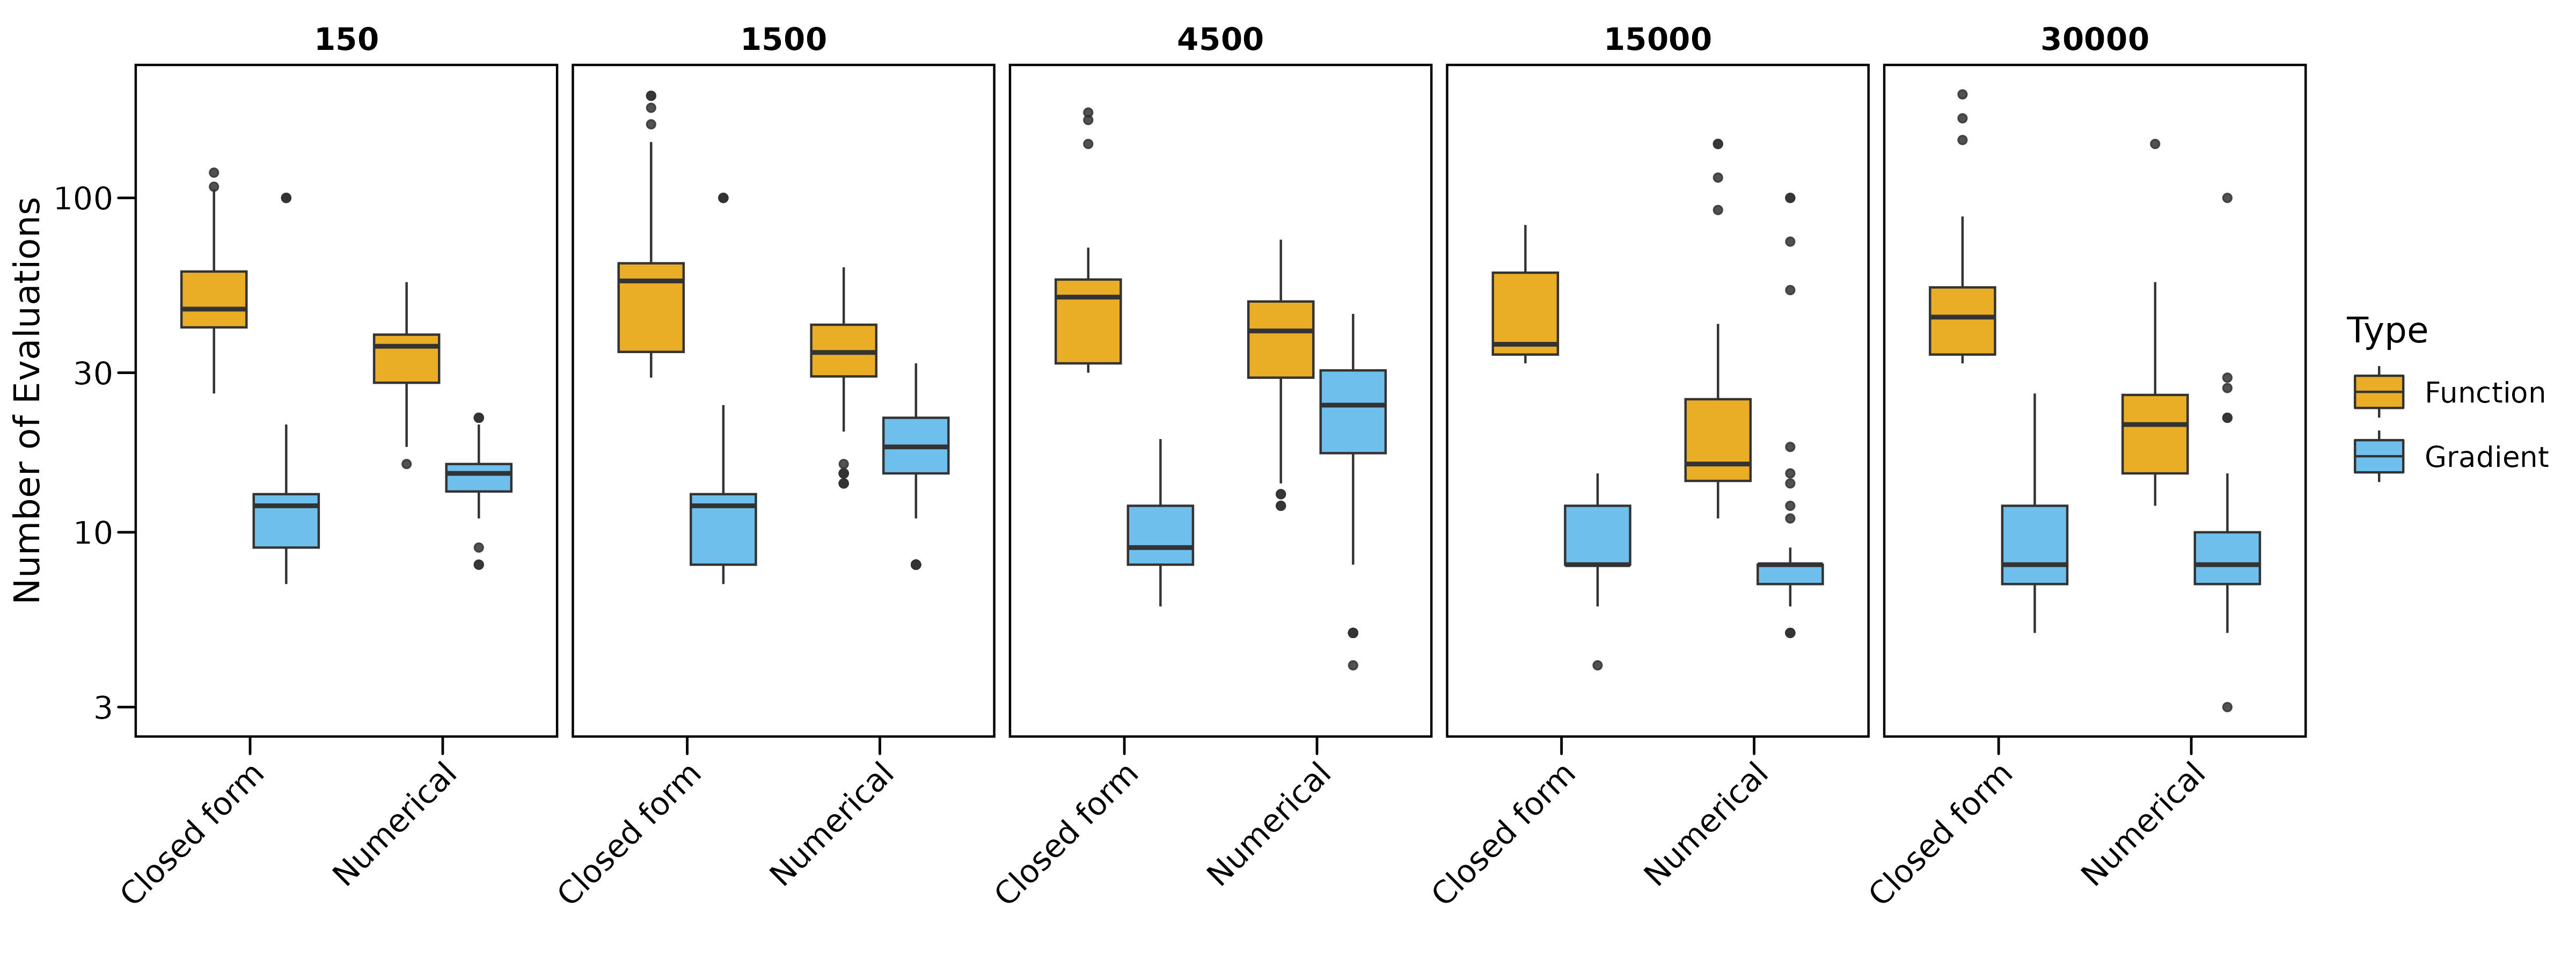
\includegraphics[scale = .08]{figures/function_gradient_count_Linear_plot.jpeg}     
    \caption{Number of gradient- and function evaluations for the two methods in the experiment on the Linear-noise model}
    \label{figure:linearFunctionGradientCount}   
    \end{center}
\end{figure}\\
Again note that to cater the reading experience we have used a logarithmic scale on the $y$-axis. A similar plot for the $F$-diffusion based model can be found in appendix \ref{section:benchmark} in figure \ref{figure:FFunctionGradientCount}; however there the difference between the methods is not as pronounced. On figure \ref{figure:linearFunctionGradientCount}, though, we see that the amount of direct function evaluations is generally higher for the closed form solution, whereas the number of gradient evaluations is a bit lower in the closed-form type Strang method. We suspect that the function-evaluations are generally less computationally heavy, because we do not supply the gradient and \code{stats::optim} thus needs to use finite-difference based methods. Albeit we cannot confirm this as we did not find a way for \code{stats::optim} to return this information to us. Although, the amount of function calls needed seems to decrease a bit for the numerical method, the shift we saw in figure \ref{figure:running_result_numeric} might stem from computation time of each call scaling better in $N$.

Of course, this example only illustrates the the numerical Strang performs better on these specific values of the parameters $\alpha_0, \mu_0, \sigma$. Still, it highlights the fact that numerical methods sometimes can achieve on par or even better performance than their closed-form counterparts. As to the specific reason for this, we let that be up to further research.
\subsection{Model misspecification}
In our final simulation study we consider how misspecifying a model can have an effect on our estimate. The way we will investigate this is simply by sampling from the additive model and fit the data with the additive- and $t$-diffusion models and consider what effect on the estimates this has. We could, of course, consider all the parameters, however as the $\tau_c$ typically is the parameter of interest, we focus on it. 

The setup of our simulations is the following: We sample using the parameters that was found on the AMOC-fingerprint data with the additive model in \cite[figure 6]{Ditlevsen2023}, i.e. $A = 0.87, m = -1.51, \lambda_0 = -2.69, \sigma = \sqrt{0.3}$. We do this with temporal resolution of $\Delta t = 1/12$ and $t_0 =54$. We vary the true value of $\tau_c$ in the values $\tau_c = \{35, 60, 90, 132, 175, 200, 250\}$. On each of theses value we run $M = 200$ experiments, where we simulate from the additive model, fit the models in the stationary parts using \cite[equation (S4-S6)]{DitlevsenSupplementary} as starting values and in the dynamical parts initialize the optimziers at the true values with the usual uniform noise. Here the noise is constructed such that the initial values deviate $\pm 15\%$ from the true values.

Note the in the fitting of the $t$-diffusion model whole idea is that we pretend that it is the true data generating distribution. As such we naturally transform the data with the lamperti-transform (see table \ref{table:ergodicDiffusions}) during the fitting of that model. For both models in all runs, we compute their uniform residuals for both the stationary- and dynamic parts. We collect the values of the empirical quantiles of them and add to them the corresponding quantiles of the standard normal distribution for comparison.

To also be able to investigate which direction an estimation might be biased we look at the relative error in the following; this is merely (\ref{eq:ARE}) without the absolute value. Due to the presence of negatiev values this means that we we cannot log-transform this graph. To cater the viewing experience, we there need remove all instances with a relative error above 1.5 in absolute value. For a quick overview of how what effect this had we tabularize the number of occurences with absolute relative error above 1.5 stratified after model true value of $\tau$. This information can be found in appendix \ref{section:benchmark} in table \ref{table:AREabove1.5tauSim}. 

We plot the distribution of the relative error for the remaining runs 
\begin{figure}[h!]
    \begin{center}
    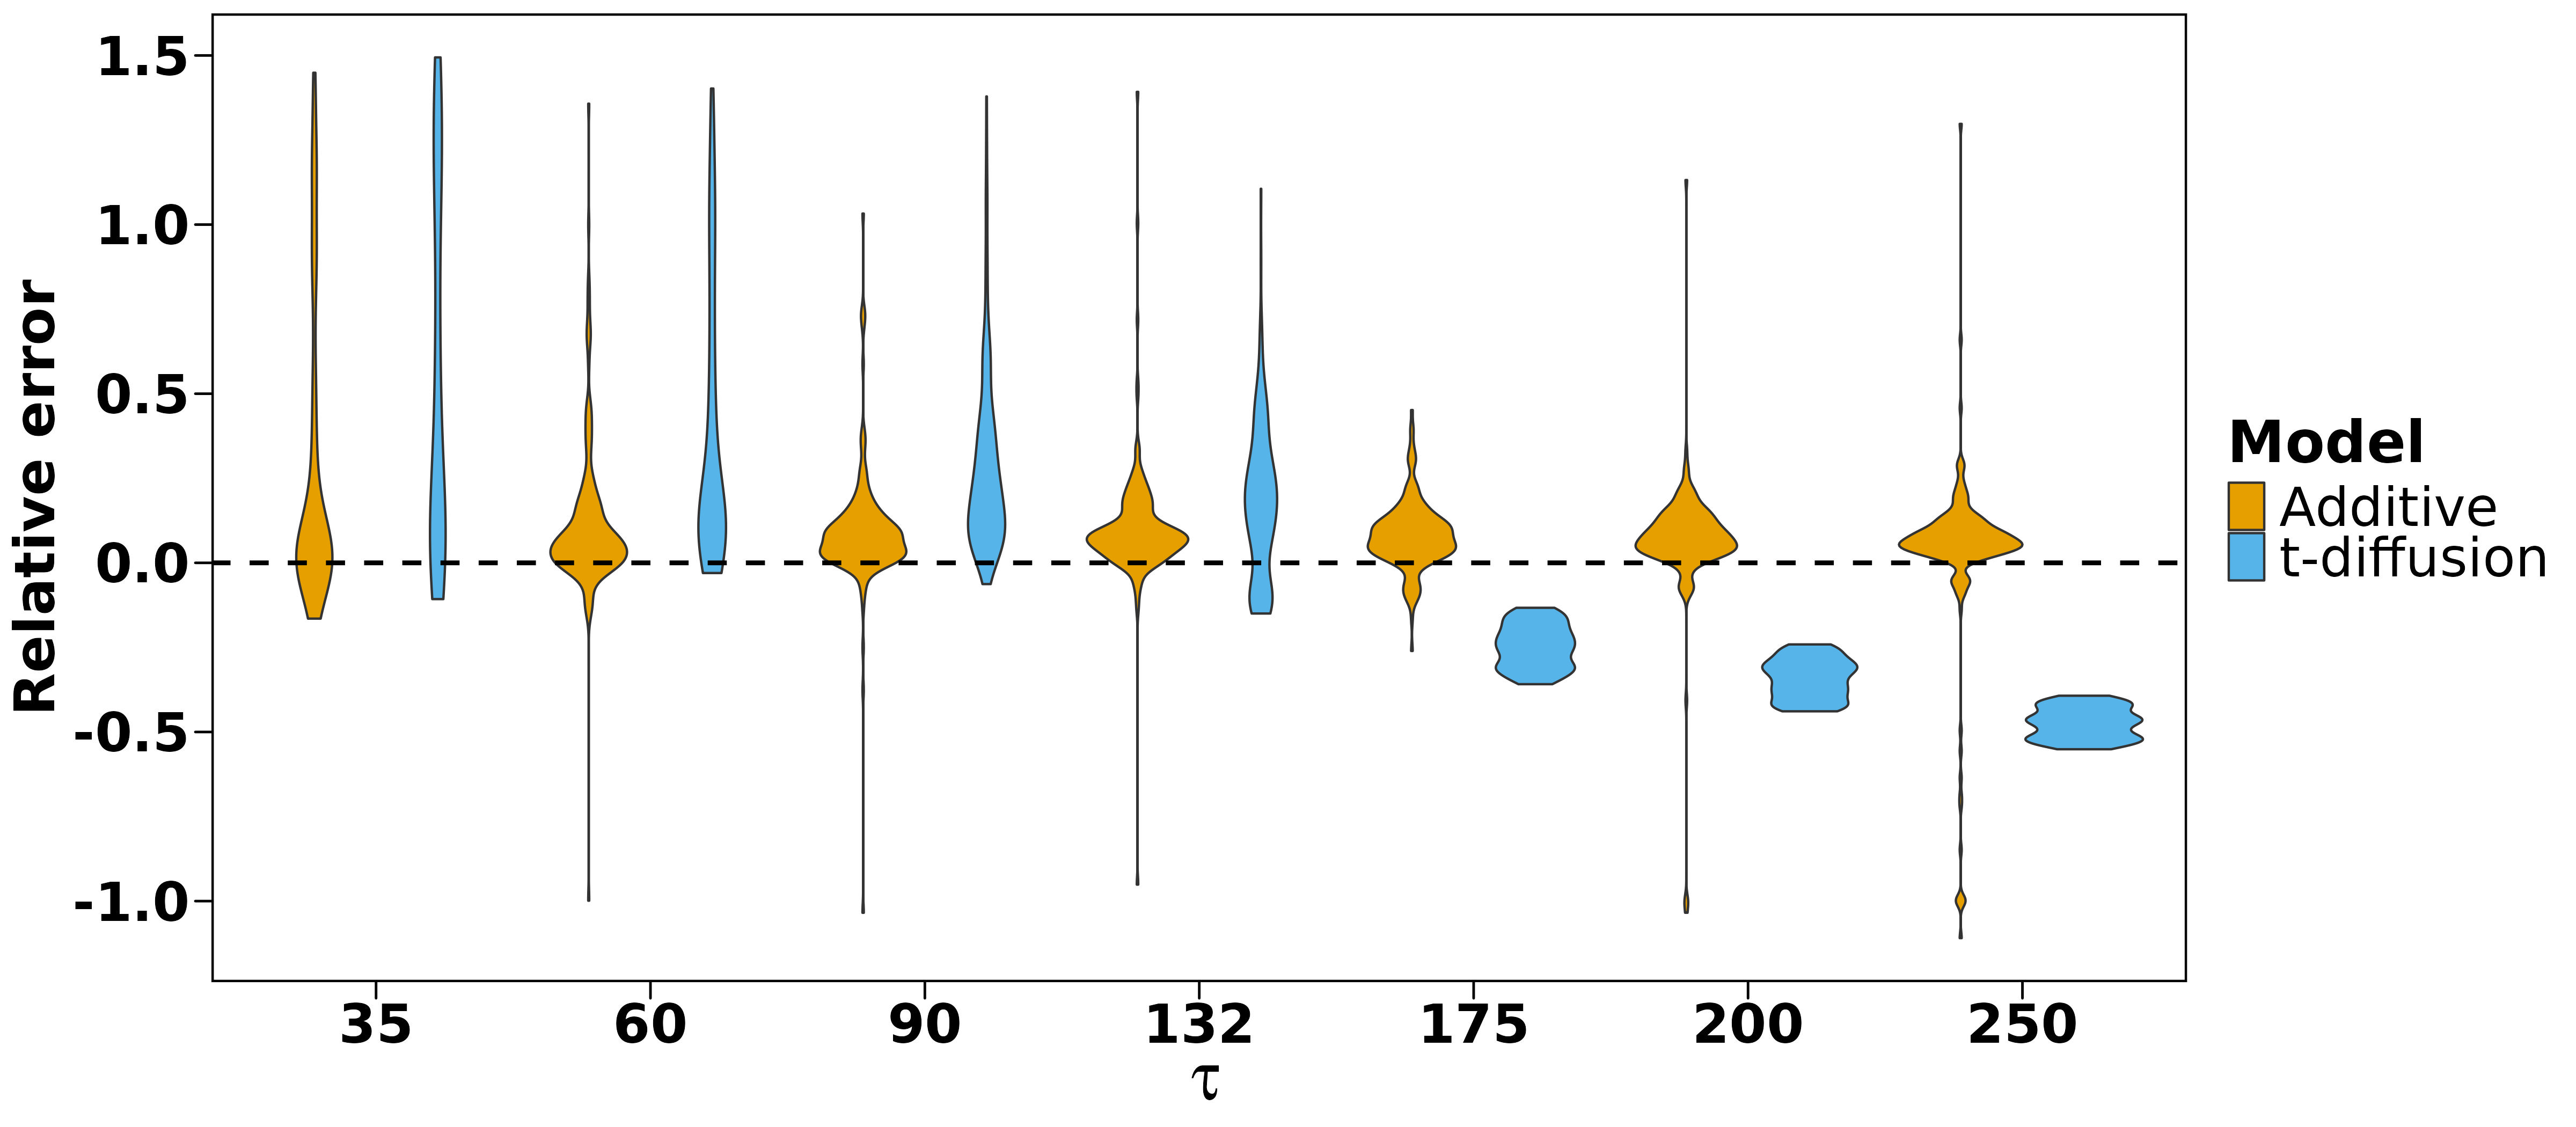
\includegraphics[scale = .075]{figures/RE_dist_tau.jpeg}
    \caption{Distribution of the relative error of the $\tau_c$-parameter stratified after the model it was fitted according to and size of the true value of $\tau_c$.}
    \label{figure:RE_dist_tau}
    \end{center}
\end{figure}\\
Interestingly, we see that the $t$-diffusion model actually estimates the tipping point alright as long as the true value is not too large. For $\tau_c = 35$ it is almost on par with the additive model. Though, generally it seems to overestimate the tipping point for smaller true values, while it underestimates it for larger true values of $\tau_c$. In addition, it seems that the additive model gets a bit biased for increasingly larger true values of $\tau_c$. The estimator based on this model, seem to overestimate the tipping a bit. 

However, the aim of this study is to mimic a real scenario a bit closer than this. In such scenarios we do not have access to the true values of $\tau_c$ and we would instead need to consider the uniform residuals. In each run we stored the range of quantiles as described above. Now, there are $80.000$ observations of pairs of $q$ and its respective $q$-empirical quantiles from these simulations and depicting the empirical quantiles in a QQ-plot with the theoretical quantiles from the normal distribution is not very insightful.

Instead, we fit a linear normal model to the empirical quantiles stratified after whether it was the additive- or the $t$-diffusion based model as well as the true value of $\tau_c$. If the models are properly specified the uniform residuals should generally lie on the identiy, and the linear regression models should reflect this
\begin{figure}[h!]
    \begin{center}
        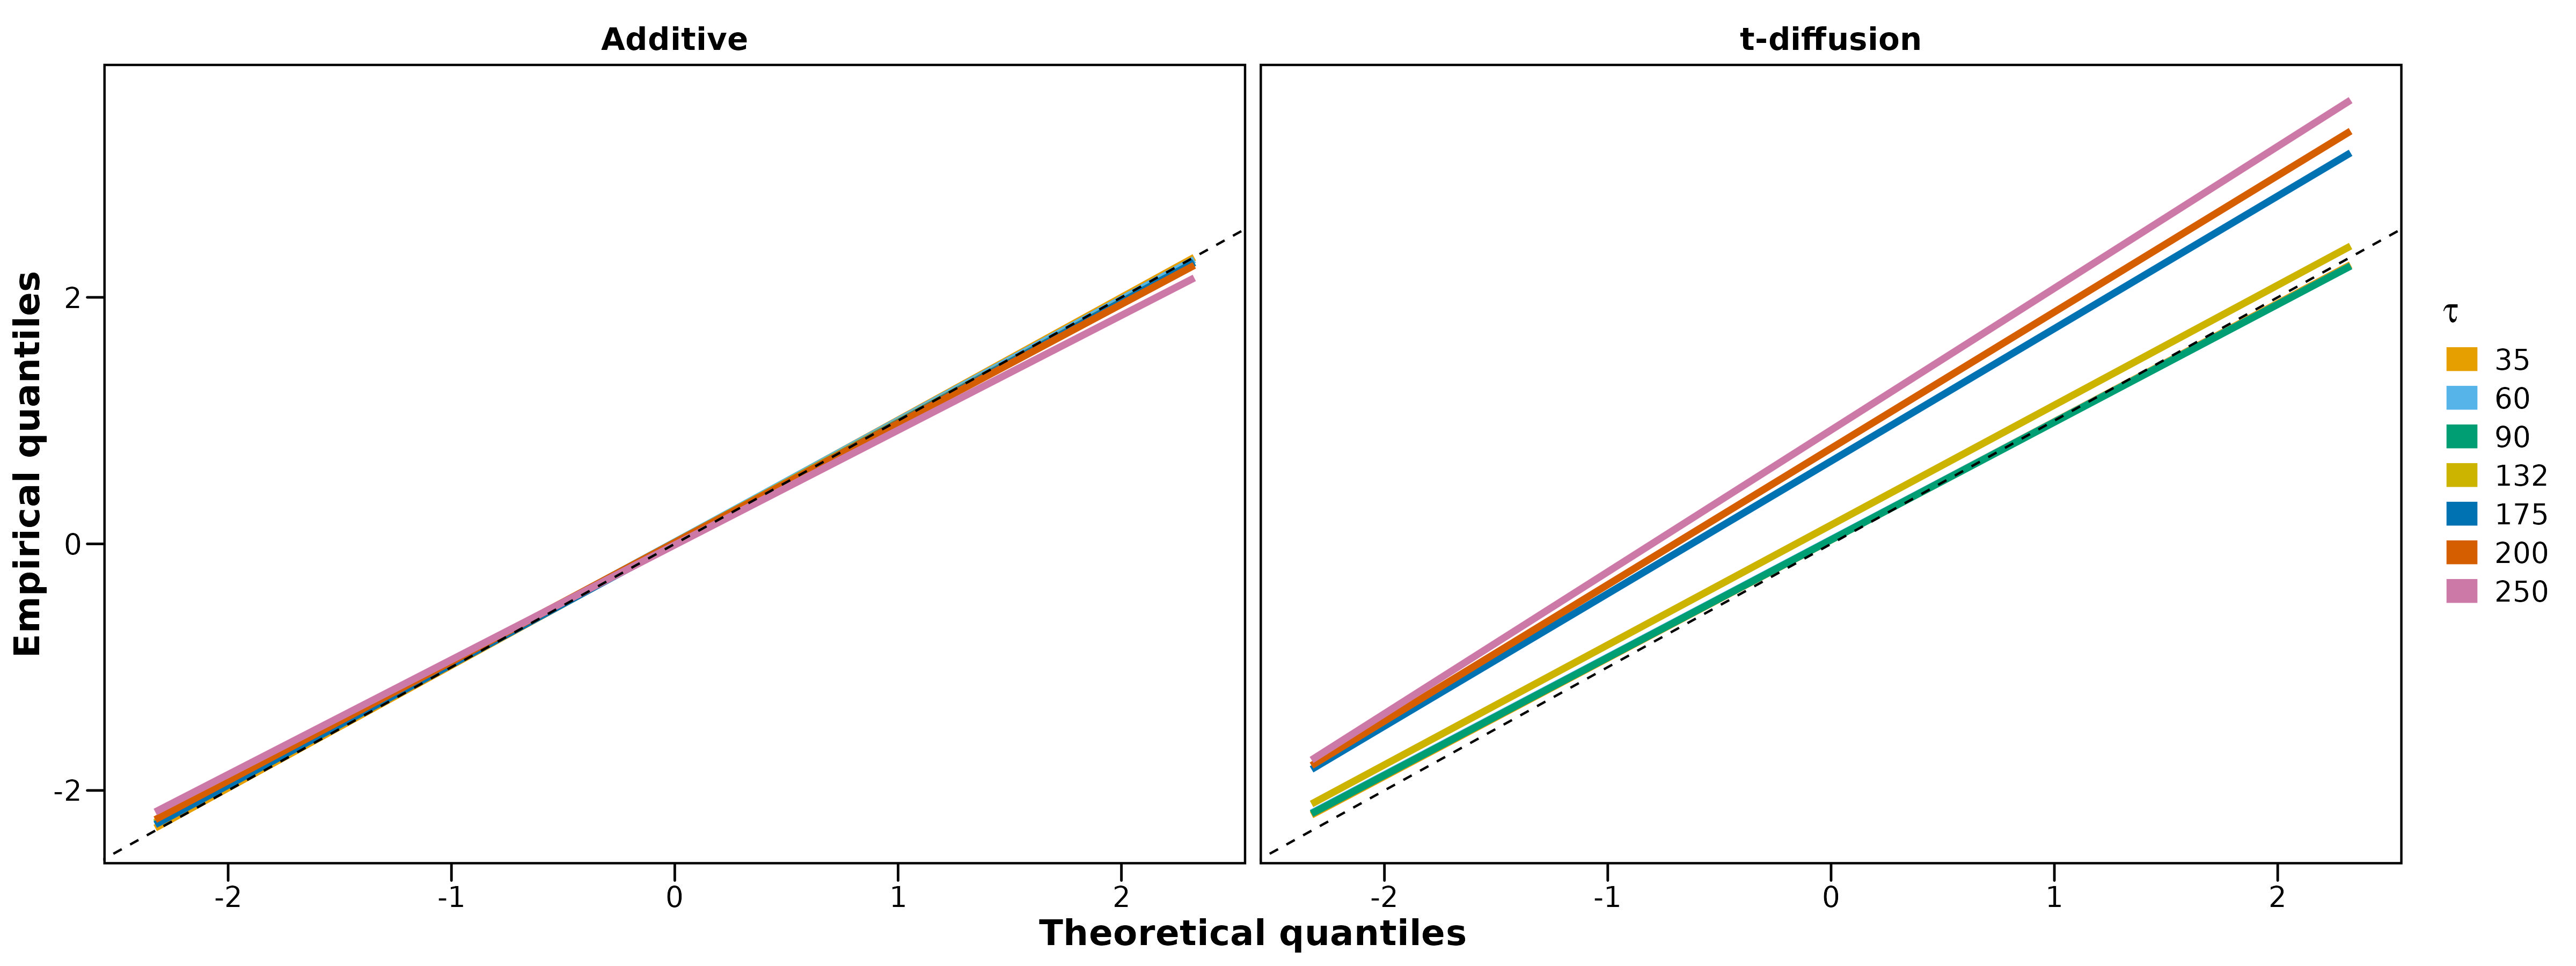
\includegraphics[scale = .075]{figures/quantiles_plot_tau.jpeg}
        \caption{Fitted linear model to data of pairs of theoretical- and empirical quantiles stratified after the true value of $\tau_c$ and the model used to fit the data.}
        \label{figure:QQ_plot_tau}
    \end{center}
\end{figure}\\
Note that the fitted lines in the $t$-diffusion facet for the true values of $\tau_c = \{35, 60, 90\}$ are almost atop one another, whence they do not appear individually in the graph. \\
The general impression across all all runs is, luckily, that it is clear from the uniform residuals that the $t$-diffusion is misspecified. However, the fit seems alright for the true values for which we also noted from figure \ref{figure:RE_dist_tau} it estimated $\tau_c$ relatively well. 